\documentclass[a4paper,11pt]{article}
\usepackage[T1]{fontenc}
\usepackage[utf8]{inputenc}
\usepackage{lmodern}
\usepackage{graphicx}
\usepackage{float}
\usepackage{enumitem}
\usepackage{pifont}
\usepackage[french]{babel}
\usepackage[a4paper, total={6in, 9in}]{geometry}
\usepackage{hyperref}
\usepackage{perpage}
\setlength{\parindent}{0in}
\renewcommand{\familydefault}{\sfdefault}
\MakePerPage{footnote}

\hypersetup{
    colorlinks,
    citecolor=black,
    filecolor=black,
    linkcolor=black,
    urlcolor=blue
}


\title{Compte rendu}
\author{
  Alexandre Legendre\\
  \and
  Eliott Sammier\\
  \and
  Vincenzo Carminati\\
  \and
  Elian Loraux\\
  \and
  Marion Chauvineau\\
  \and
  Lucas Lacouture\\
}

\begin{figure}[H]
  
\includegraphics[width=500px]{images/page-de-garde.png}
  \label{fig:mpage-de-garde}
\end{figure}

\begin{document}

\newpage
\tableofcontents
\newpage

%==============================================================================
%                           CADRAGE DU PROJET
%==============================================================================

\section{Cadrage du projet}

%---------- description ----------

\subsection{Description du projet}
En cette période de crise sanitaire, et notamment durant le confinement, nous avons pu observer une
émergence de la solidarité entre voisins. Au sein d’un immeuble, d’une rue ou bien d’un quartier,
certains voisins ont œuvré pour une ambiance conviviale, voire familiale, afin d’apporter un soutien en
cette période. Au travers de concerts improvisés, de cours de sport ou même de variantes de jeux
télévisés “Question pour un champion” transformé en “Question pour un balcon”,
une certaine fraternité entre voisins a vu le jour. Récemment, les grandes crues dévastatrices dans le Sud-
Est ont soulevé un élan de solidarité. La finalité de notre projet serait de donner un cadre à cette
entraide pour pouvoir la rendre plus régulière et plus simple à mettre en place.
Durant cette période de crise sanitaire, cela prend du sens notamment pour la mutualisation des
courses. Prenons l’exemple d’une personne fragile : à la place d’aller faire ses courses elle-même et
d’être par conséquent en contact avec tous les clients du magasin, elle n’est qu’en contact avec un
voisin. Inversement, pour une personne atteinte ou avec des suspicions de Covid-19, cela limite les
contacts et par conséquent les risques de transmission.\\

Notre projet est un service de mise en relation et d’échange de services entre particuliers à proximité.\\

Il prendra la forme d’un site Web. L’utilisateur pourra demander, consulter et répondre à un service.
Les services iront de la garderie aux petits travaux en passant par le dépannage informatique, ou
même des courses régulières. L’idée est de faire une plateforme participative et diversifiée grâce aux
compétences individuelles de chaque utilisateur.\\

%---------- Objectifs ----------

\subsection{Objectifs}

\underline{Simplifier l'entraide}\\

L'objectif principal est de simplifier l'entraide entre voisins.
Cette simplification entraînera une pérennisation et une diversité des services.
En proposant des sondages et des questionnaires à nos inscrits, nous pourrons évaluer si notre site facilite effectivement l'entraide et à quel point.\\

\underline{Facilité d'utilisation}\\

Le voisinage est un des meilleurs exemples de mixité sociale.
On y trouve des jeunes, des personnes âgées, des ouvriers, des ingénieurs, des familles, autant de personnes qui sont plus ou moins à l'aise en informatique.
C'est à nous de nous adapter à tous ces différents niveaux. Il faut donc que le site soit simple et facile d'utilisation.
Pour atteindre cet objectif, nous pouvons assurer un guidage sur le site en suivant les règles d'accessibilité du W3C et faire une foire aux questions par exemple.\\

\pagebreak

\underline{Des utilisateurs de confiance}\\

Selon les services, on peut avoir besoin d'utilisateurs de confiance.
Par exemple, pour des travaux de plomberie, il faut quelqu'un capable de réparer et surtout de ne pas empirer les dégâts ; ou encore, pour les personnes âgées, il faut que les personnes qui interviennent au domicile ne soit pas mal intentionnées.
Il est donc important de vérifier les utilisateurs.\\
Nous avons retenu trois critères à vérifier : la fiabilité (réputation), l'identité et les compétences de l'utilisateur.\\


%---------- Description du contexte ----------

\subsection{Description du contexte}

Il existe plusieurs sites fournissant des services similaires à ceux de notre projet, les principaux étant :\\

\begin{itemize}
  \item \textbf{AlloVoisins}\footnote{\url{https://www.allovoisins.com/}} : propose un service de mise en relation entre particuliers avec 3,5 millions d'utilisateurs. La grande majorité des annonces y sont rémunérées, l’option non rémunérée
  n’étant que très peu utilisée. Certaines entreprises sont aussi présentes sur le site.

  \item \textbf{Pwiic}\footnote{\url{https://pwiic.com/fr/}} : c’est un site qui permet d’échanger des services ou objets auprès de particuliers. Il suffit d’envoyer un “Pwiic” pour que la demande s’affiche sur le site. Un algorithme se charge de
  l’envoyer aux bonnes personnes.

  \item \textbf{YakaSaider}\footnote{\url{https://www.yakasaider.fr/}} : c’est un site communautaire qui met en relation des particuliers proposant ou ayant besoin d'un service. Il se base sur un crédit horaire : pour chaque heure passée à rendre des services, l’utilisateur a le droit de demander une heure de service.
\end{itemize}

Nous avons comparé ces sites sur la base de critères simples (figure 1).\\
Pour les services proposés, nous avons choisi le prix ou la gratuité pour comparer notre service aux leurs.
Notre service se veut basé sur le bénévolat ou l'échange. Seul Pwiic propose ceci.
Il nous fallait donc d'autres critères, comme l'ergonomie ; en effet, notre site se veut facile d'utilisation.
Nous avons donc observé le guidage et la gestion d'erreurs, étant donné que les autres sites du marché ne semblent pas suivre de norme. Art Entraide se distinguera en suivant les normes W3C en matière d'ergonomie.\\
Et enfin, le critère sur lequel nous voulons nous démarquer : la certification.
Peu de sites possèdent un système de certification, et même quand c'est le cas, il est relativement facilement contournable et n'apporte pas de véritable protection.
Nous voulons mettre en place un système où la vérification se fera par des institutions, des mairies ou des associations, de telle sorte que la certification soit un gage de confiance.\\

\begin{figure}[H]
  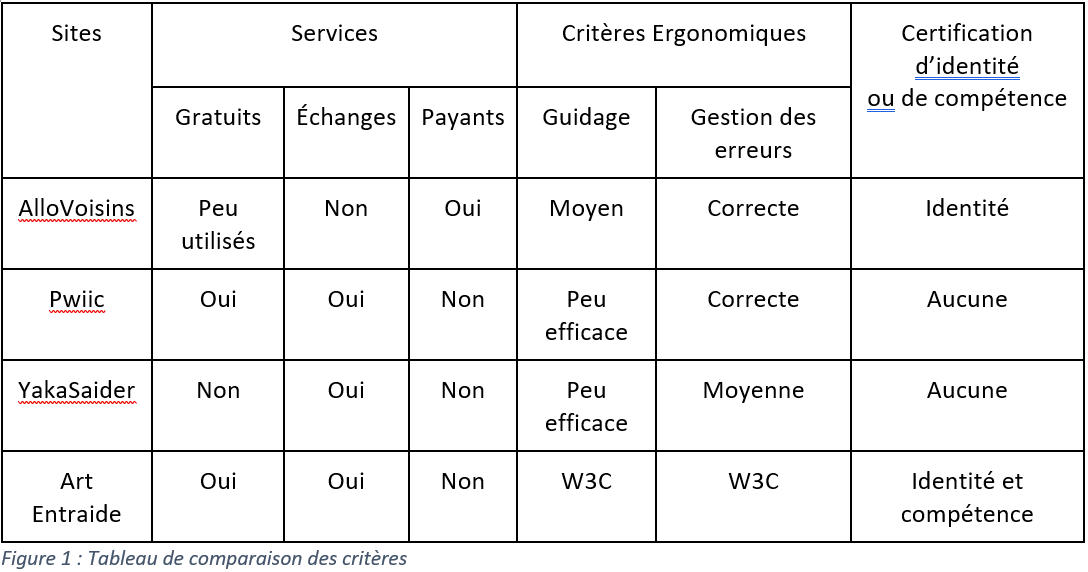
\includegraphics[width=\linewidth]{images/tableau-ergo.png}
  \caption{Tableau de comparaison des critères.}
  \label{fig:table1}
\end{figure}

Le marché a donc une limite claire. L'utilisateur n'a pas de moyen concret de savoir si la personne avec qui il communique est réellement qualifiée, ou même existe.
Art Entraide veut apporter ce moyen.\\

Une description plus poussée des sites est disponible en annexe.\\

%---------- Acteurs du projet ----------

\subsection{Acteurs du projet}
\subsubsection{Maîtrise d’ouvrage}

Le domaine d’activité visé est la mise en relation et l’échange des services pour particuliers.\\

Les enseignants sont ceux qui ont commandé le projet, par l’intermédiaire du sujet.\\

Les utilisateurs seront des personnes à risque, des personnes âgées ou simplement des particuliers
voulant échanger des services. Ils s’attendront à pouvoir demander et proposer des services
simplement à des personnes à proximité.\\

\subsubsection{Maîtrise d'œuvre}

Elle est composée de 6 étudiants en deuxième année de DUT Informatique, qui s’occuperont de définir les
besoins, de concevoir et réaliser une solution.\\

\subsubsection{Intervention de sous-traitants}

Les sous-traitants possibles sont des associations ou des mairies pour vérifier l’identité des utilisateurs
bénévoles.\\

%---------- Contraintes ----------

\subsection{Contraintes}

Notre projet est affecté par l’environnement actuel, les conditions sanitaires, le public cible, etc...
Le cadre du projet définit donc un certain nombre de contraintes.

\subsubsection{Contrainte temporelle}

Pour ce projet, la contrainte temporelle est forte. En effet, le déroulé se présente sous forme de
3 itérations successives (le 13 octobre 2020, le 24 novembre 2020 et le 15 janvier 2021) avec pour
chacune une date de rendu de dossier et d’évaluation.\\

La charge totale attendue est d’environ 950 heures et nous disposons de 17 semaines (vacances
comprises) pour réaliser ce projet.\\

\subsubsection{Contrainte sanitaire}

À la suite de la deuxième vague de la crise sanitaire du COVID-19, la contrainte sanitaire s'est renforcée.
En effet, toutes les séances de projet sont désormais en distanciel.\\

Cela pose donc la question du travail à distance. En effet, à présent la totalité du travail doit être effectué à distance. Nous devons donc utiliser des outils informatiques pour continuer à échanger des
informations, discuter de l’avancée du projet, répartir les tâches etc...\\

\subsubsection{Contrainte matérielle}

Le travail à distance implique aussi une contrainte matérielle. En effet, les membres du groupe doivent
avoir un minimum de matériel informatique pour pouvoir travailler depuis chez eux.\\

Les membres du groupe sont-ils tous dans de bonnes conditions pour travailler correctement à
distance ? Au minimum, il faudra un ordinateur pour développer le site, ainsi qu’une connexion
Internet.\\

\subsubsection{Contrainte juridique}

La création de compte sur le site implique le stockage des données personnelles de l’utilisateur. Ces
données pouvant être sensibles, telles que des adresses ou des mots de passe, elles sont soumises à
certaines lois, notamment le règlement général sur la protection des données (RGPD). Nous devrons donc nous
conformer à ces dernières, c'est donc une contrainte juridique.\\

\pagebreak

\subsection{Risques}

Durant la réalisation ce de projet, il est possible que ce dernier ne s’exécute pas comme prévu. Il nous
faut donc tenter d’identifier ces risques et mettre en place un plan de mitigation.\\

\subsubsection{Risque temporel}

Une mauvaise organisation des membres du groupe peut entraîner un retard. Cette éventualité est
probable et son impact serait critique. En effet, nous pourrions accumuler ce retard, or les échéances
successives nous en empêchent. La criticité de ce risque est donc substantielle.\\

Une mauvaise compréhension des besoins est un évènement probable. Pour les mêmes raisons
qu'une mauvaise organisation, ce risque a un impact critique. Sa criticité est donc substantielle.\\

Il est également possible qu'un membre du groupe tombe malade et soit dans l'incapacité de travailler, ou avec une efficacité réduite. En période de confinement, ce scénario est peu probable, mais son impact
serait majeur puisqu'il impliquerait une redistribution du travail et une hausse de charge pour les autres membres. C'est un risque modéré.\\

\subsubsection{Risque matériel}

La perte de documents est probable, une feuille égarée ou un disque dur défaillant sont des choses
qui peuvent arriver. Il est probable que ce risque survienne et son impact serait critique car le travail
devrait être refait, ce qui serait une perte de temps, une ressource précieuse dans
ce projet. Sa criticité est alors substantielle.\\

\subsubsection{Risque judiciaire}

L’utilisation du site pour des actes malveillants est une éventualité probable et son impact serait
majeur car cela pourrait mettre en danger les utilisateurs. Sa criticité est donc substantielle.\\

\subsubsection{Plan de mitigation}

Pour la perte de documents, nous choisissons la protection : nous mettrons en place une redondance
des documents en numérisant tous les documents physiques et en les stockant dans le cloud, ainsi
que sur le disque dur d’au moins deux de nos machines. Le code sera hébergé sur le dépôt Gricad-Gitlab ainsi que sur chacune de nos machines.

Enfin, par rapport à l’utilisation du site pour des actes malveillants, nous transférerons le risque à des
associations ou des mairies avec qui nous traiterons pour certifier les utilisateurs du site.

Concernant la mauvaise organisation du groupe, nous prenons une statégie de réduction. Nous nous organiserons
à l'avance et en se concertant tous ensemble. Si malgré cela l'organisation est mauvaise, nous
assumerons les pertes de temps. Quant à la mauvaise compréhension des besoins, nous choisissons
aussi une statégie de réduction. Nous poserons des questions à la maîtrise d'ouvrage et nous pourrions aussi sonder
les clients.\\

\newpage

%==============================================
%         Expression du besoin
%==============================================

\section{Expression du besoin}

Pour mieux cerner les fonctionnalités et les besoins auxquels nous devons répondre, nous avons créé un diagramme de cas d'utilisation.
Celui-ci sera explicité dans les prochaines sous-parties.

\begin{figure}[H]
  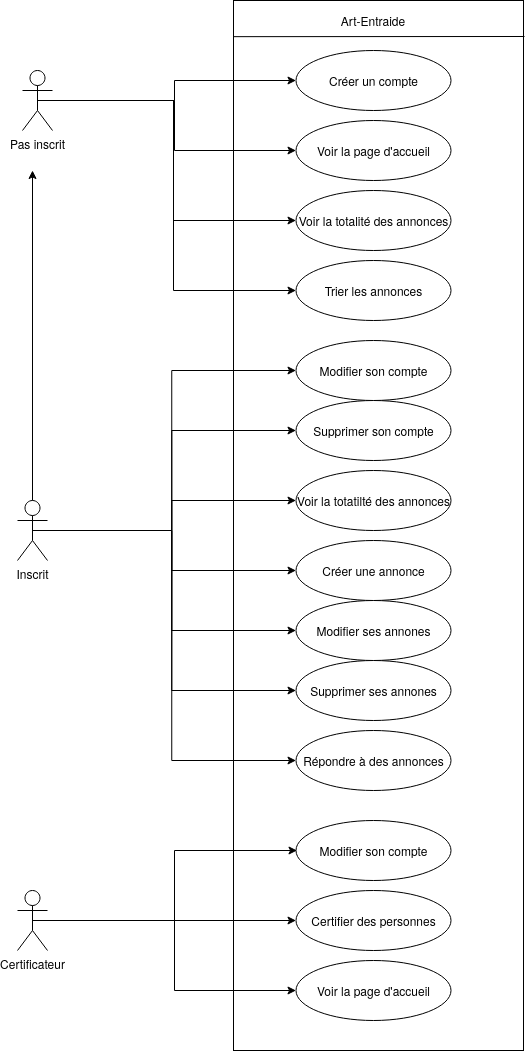
\includegraphics[width=250px]{../Conception/DCU.png}
  \caption{Diagramme des cas d'utilisation}
  \label{fig:DCU}
\end{figure}

%---------- Besoins fonctionnels ------------

\subsection{Besoins fonctionnels}

Le site devra permettre une mise en relation entre les particuliers (c’est sa fonction principale). Il
permettra ainsi à des individus proches géographiquement de se rencontrer pour pouvoir s’entraider
sur différents types de tâches.\\

\subsubsection{Annonces}

Afin de mettre en relation les particuliers, le site permettra la création d'"annonces", correspondant à une recherche ou proposition de service.\\

Ces annonces seront accessibles à la consultation au public, et les utilisateurs intéressés par une annonce pourront y répondre et être directement mis en contact avec l'auteur de l'annonce.

\subsubsection{Comptes }

Afin de permettre d'identifier les différents utilisateurs sur le site, un système de comptes, que l'on pourra créer et gérer, et auxquels seront associées les actions faites par chaque utilisateur (création d'annonce, réponse aux annonces, messages, etc...), devra être mis en place.

\subsubsection{Certification des utilisateurs}

Pour vérifier la fiabilité des utilisateurs, nous avons pensé à un système de réputation avec un score numérique, qui serait un premier critère de confiance.\\

Pour la vérification de l'identité, les utilisateurs pourraient se faire certifier via un tiers comme une mairie ou une association.\\

Et le moyen pour la vérification des compétences n'est pas encore défini avec exactitude, mais nous envisageons une certification par diplômes (liée aux mairies notamment) et/ou la certification de compétence par les usagers.
Si X personnes, après avoir bénéficié d'un service de la part d'un certain utilisateur, attestent que cet utilisateur est qualifié, alors la certification peut être donnée.
Il faut néanmoins faire attention à ne pas certifier quelqu'un qui n'a pas les compétences.\\

\subsubsection{Différents types de comptes}

Le site doit permettre la création de comptes pour les utilisateurs, mais également de comptes
pour les certificateurs, c'est à dire les organisations mentionnées ci-dessus chargées de vérifier l'identité et les compétences des utilisateurs.\\

Étant donné que ces comptes certificateurs auront la capacité de certifier d'autres comptes (une responsabilité importante), une authentification plus complexe devra être mise en place pour s'y connecter.\\

\subsubsection{Localisation}

Afin de pouvoir proposer à l'utilisateur uniquement les offres proches de chez lui, il faut que l'on
puisse trier les annonces par leur localisation.\\

Il sera donc nécessaire, au moment de l'inscription d'un utilisateur ou de la consultation d'annonces, d'enregistrer sa localisation
géographique, afin de lui proposer des annonces proches et, vice-versa, de proposer ses annonces aux gens proches de lui.\\

On pourra récupérer la localisation de l'utilisateur par plusieurs moyens:\\
\begin{itemize}
  \item Demander simplement la saisie d'une adresse
  \item Récupérer la localisation de l'appareil via la permission du navigateur.
\end{itemize}

%---------- Besoins non fonctionnels ------------

\subsection{Besoins non fonctionnels}

\subsubsection{Critères qualité}

\textbf{Sécurité}\\

Les données que les utilisateurs nous confient, tels que leur adresse, numéro de téléphone, etc... sont
sensibles : une certaine sécurité doit donc être assurée.\\

Il faudra donc mettre en place un système d'authentification aux comptes mentionnés plus haut.\\

On pourra ou bien se connecter via un système d'authentification programmé par nos soins, ou bien via l'API de login fournie par Google pour permettre aux utilisateurs de se connecter sur le site via leurs comptes Google, ce qui aurait également l'avantage de la simplicité (un grand nombre de personnes utilisent un compte Google).\\

Il faudra aussi s'assurer que la partie logique du site soit stockée côté serveur, et de n'envoyer à la machine de l'utilisateur que les informations auxquelles il est censé avoir accès.\\

\textbf{Échelle du projet}\\

Pour commencer, nous voudrions mettre en place un site permettant de gérer au minimum une centaine de comptes et annonces simultanément.\\

\subsubsection{Critères ergonomiques}

Étant donné que le public visé par ce projet est très large, le site doit être accessible et utilisable par
tous types de personnes majeures. Cela inclut donc les personnes qui ne sont pas familières avec Internet, ou
avec les ordinateurs en général. Il est donc nécessaire de rendre le site le plus accessible et simple d'utilisation
possible, en suivant notamment les critères ergonomiques de Bastien et Scapin.\\

\textbf{Guidage}\\

Pour faciliter l'utilisation du site aux utilisateurs et éviter qu'ils ne se retrouvent perdus, ils sera important dans le design des pages du site, de s'assurer de bien disposer les informations essentielles au centre et en haut de la page, afin que ce soit la première chose que l'utilisateur voie sans avoir besoin de \textit{scroller}.\\

Il est important que l'utilisateur n'ait pas à se demander ce que l'on attend de lui, dès l'instant où il pose ses yeux sur la page, ce qu'il doit faire est clair.

Les textes devront être adaptés à l’utilisateur, par exemple si ce dernier a des problèmes de vue.

Il sera donc nécessaire de choisir des polices d’écritures simples à lire, de s’assurer que sa taille soit
réglable via le navigateur, d’utiliser un contraste et des couleurs adaptés.

Il faut également prendre en compte d’éventuels daltoniens qui pourraient utiliser le site, en
choisissant des couleurs assez différentes.\\

\textbf{Charge de travail}\\

Il faudra en même temps éviter de surcharger ce haut de page, et n'y laisser que les informations essentielles, afin d'éviter de surcharger l'utilisateur d'informations.\\

\textbf{Cohérence}\\

Les informations du site doivent être présentées de la même façon à chacune de leurs apparitions, afin de les rendre plus compréhensibles pour l'utilisateur.

Par exemple, la catégorie d'une annonce, si elle est représentée sur une page par une icône, ou écrite d'une certaine couleur, devra être représentée de la même façon sur toute les autres pages du site.


%---------- Fonctions attendu ------------

\subsection{Fonctions attendues}

\subsubsection{Création d’annonces}

Notre site doit permettre aux utilisateurs de mettre en ligne des annonces créées par leurs soins. Cela
peut être une annonce de recherche d’aide, ou une annonce pour au contraire proposer de l’aide. Le
site doit également permettre aux utilisateurs de personnaliser leurs annonces, en choisissant le type
de travail fourni/demandé, en ajoutant une description, et en précisant d’autres détails, tels que la date, le
niveau d’expertise demandé ou une estimation de durée.\\

\subsubsection{Recherche d’annonces}

Une page de recherche d’annonces sera disponible sur le site, et permettra aux utilisateurs de
rechercher des annonces correspondantes à leurs attentes. Ils pourront trier les annonces par
localisation, par date, par catégorie, et par type (proposition ou demande). Une fois que l’utilisateur
a trouvé une annonce qui l'intéresse, il pourra ensuite entrer en communication avec celui qui a
publié l’annonce via un chat textuel.\\

\subsubsection{Gestion de comptes}

Le site demandera aux utilisateurs de créer un compte avant de pouvoir créer ou répondre à des
annonces. Une page permettra de se connecter à son compte et une autre de gérer ses informations
personnelles.\\

\newpage

%=============================================
%                 SOLUTIONS
%=============================================

\section{Solutions}

\subsection{Spécifications détaillées}

\subsubsection{Conception ergonomique}
\paragraph{Maquette}\mbox{} \\

A titre d’exemple, voici une page qui préfigure l’ergonomie qui s’appliquera au site. Le reste des maquettes ainsi que les toutes premières se trouve en \underline{\hyperref[sec:maquettes-annexe]{annexe}}. Les différentes pages doivent rester
simples en termes de composants, avoir des couleurs sobres et claires afin d’être compréhensibles
par le public ciblé, notamment des personnes âgées.\\

\begin{figure}[H]
  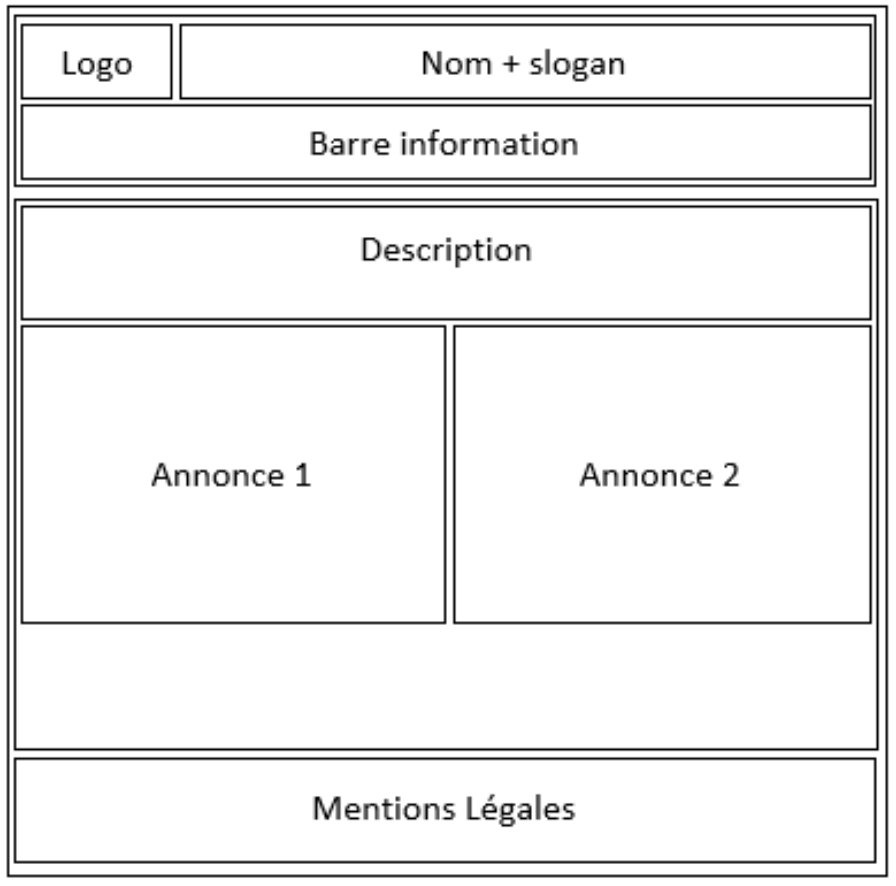
\includegraphics[width=\linewidth]{images/maquette-accueil.png}
  \caption{Page d'accueil.}
  \label{fig:maquette-accueil}
\end{figure}

\pagebreak

\subparagraph{En-tête}

L'en-tête est composé du logo du site, d'une barre de recherche et de 3 boutons.
Avec seulement 5 éléments, nous réduisons la densité informationnelle.\\
La barre de recherche et le bouton "Catégories" servent tous les deux à rechercher une
annonce, l'un avec des mots-clés, l'autre en filtrant par catégorie, renforcant
la flexibilité.\\


Si l'utilisateur est déjà connecté, les boutons "Se connecter" et "S'inscrire"
sont remplacés par le nom de l'utilisateur et son icône de profil, qui seront
cliquables afin d'accéder aux paramètres de son compte.\\

\subparagraph{Page d'accueil}

La page d'accueil est composée d'une courte description du site, de quatre annonces et
d'un bouton permettant d'atteindre la page d'affichage/filtrage des annonces.
Le fait d'avoir uniquement une courte description et ces quatre premières annonces
dès l'arrivée sur le site renforce l'incitation, expliquant tout de suite à quoi sert
le site.\\

Les sections représentant les annonces comportent les informations importantes des
annonces, notamment leur titre, leur catégorie et un badge présent près de la photo de profil
de l'auteur de l'annonce témoignant de sa certification s'il en a une. La catégorie d'une annonce
est en fait un bouton permettant d'accéder à toutes les annonces de la même catégorie,
renforcant encore une fois la flexibilité avec le l'en-tête ; de plus, l'encadré entier de l'annonce
est aussi un lien menant vers le détail de l'annonce.\\

\paragraph{Évaluation ergonomique}\mbox{} \\

Les principaux critères ergonomiques auxquels notre IHM va se conformer sont :\\

\begin{itemize}
  \item Le \textbf{guidage} : un fil d’Ariane toujours visible sur le haut de l’interface permettra aux utilisateurs de
  se repérer facilement dans le site et sur les actions en cours. Une illustration des actions
  possibles et des formulaires sur le panneau central du site facilitera l’accès aux différents
  services. Les éléments cliquables auront également des infobulles au survol qui préciseront leur fonction.
  \item Le \textbf{contrôle explicite} : la suppression des offres de service sera protégée par une double
  demande, et la mise en relation sera explicite afin de protéger les utilisateurs.
  \item La \textbf{prévention des erreurs} : un contrôle local sera mis au niveau de chaque champ pour vérifier que
  les données entrées par l'utilisateur sont conformes (format email, tel ...) avec un sticker \textit{check} vert
  dès que le champ est valide. Pour tous les champs qui s'y prêtent, la saisie se fera par menu déroulant, boutons radio ou cases à cocher plutôt que par champ texte libre pour limiter les risques d'erreur de saisie.
  \item La \textbf{gestion des erreurs} : un pop-up sera mis en place pour permettre un guidage des
  utilisateurs en cas d’erreur de saisie et en particulier pour aider les personnes âgées.
  \item La \textbf{charge de travail} : la création des offres se fera avec un formulaire, afin de limiter les étapes
  nécessaires à l’enregistrement grâce à un pré-remplissage des champs -- lorsque cela est possible --
  avec les informations de compte de l’utilisateur lorsqu’il est authentifié. La recherche des
  offres sera également simplifiée, avec l’utilisation des préférences de l’utilisateur pour
  pré-remplir les champs de recherche.
  \item La \textbf{cohérence interne} : chaque page sera la plus similaire possible aux autres pour faciliter
  l'apprentissage du site et ne pas se sentir perdu.
  \item La \textbf{flexibilité} : pour faciliter l'utilisation du site, il y aura souvent plusieurs actions possibles
  pour arriver à faire la même chose.
  \item L'\textbf{adaptabilité} : compte tenu du public visé, nous allons mettre en place un mode spécifique
  pour les personnes malvoyantes, activant une adaptation de taille et contraste de police pour
  une meilleure accessibilité.
\end{itemize}

Lors de la réalisation des maquettes, nous avons essayé de respecter ces critères au maximum.
Par exemple, pour la cohérence interne, l’en-tête et le pied de page sont communs à toutes les pages du site.

\paragraph{Plan du site}

\begin{figure}[H]
  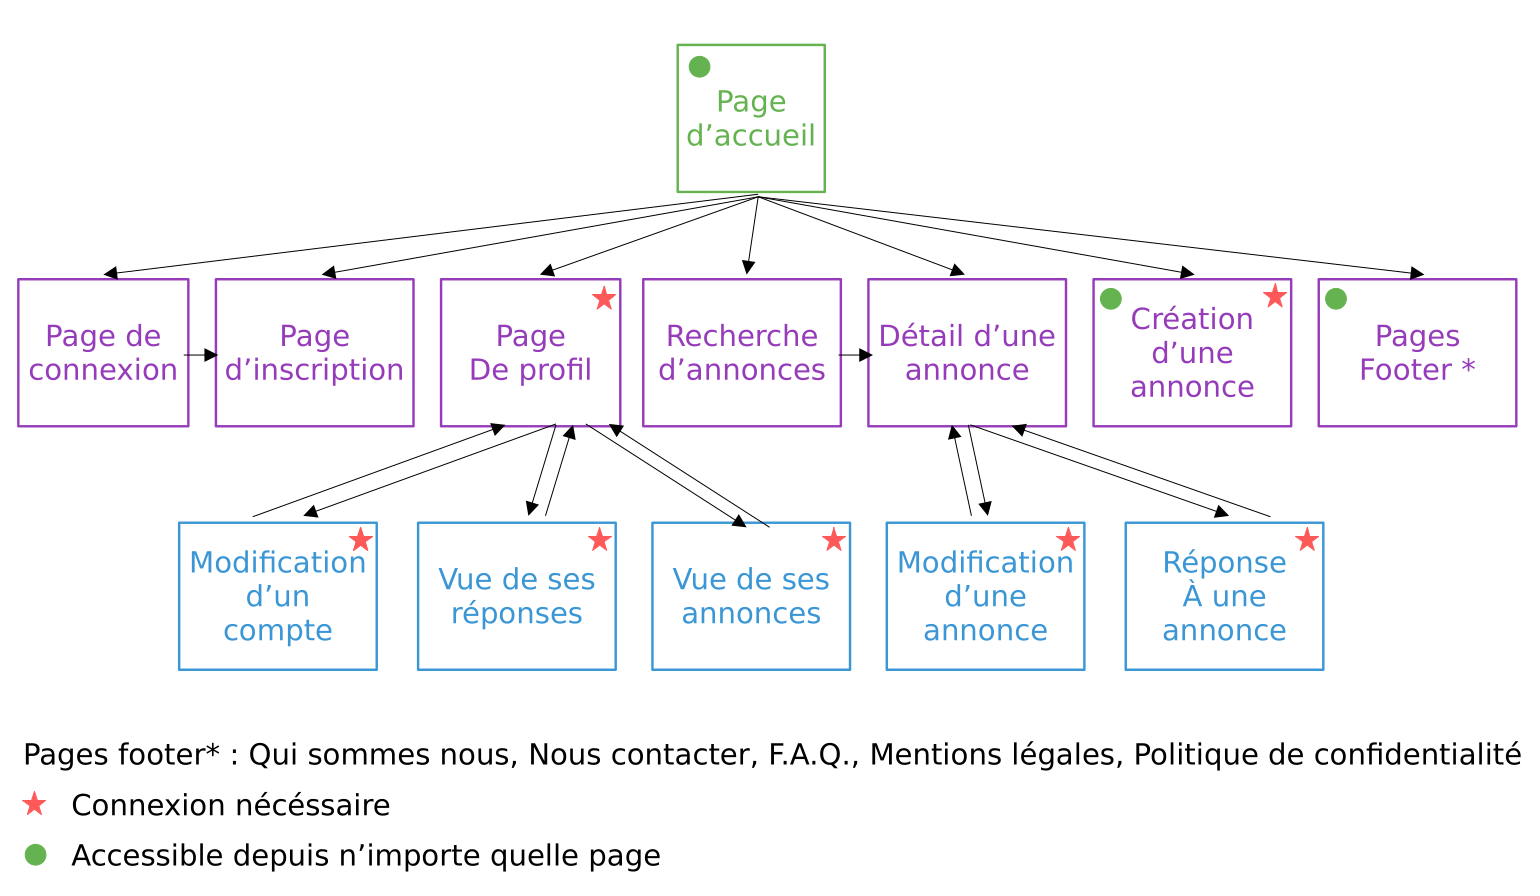
\includegraphics[width=\linewidth]{images/plan-du-site.png}
  \caption{Plan du site}
  \label{fig:plan-du-site}
\end{figure}

Voici une représentation simple du plan du site. L'utilisateur pourra rechercher rapidement une annonce
à n'importe quel moment grâce à la barre de recherche dans l'en-tête.

Si l'utilisateur va sur la page de connexion alors qu'il n'a pas de compte, il peut directement
accéder à la page d'inscription sans passer de nouveau par l'accueil.

Depuis chaque page, l'utilisateur pourra accéder aux pages d'un niveau inférieur grâce au fil d'Ariane
mais il pourra aussi retourner à la page d'accueil à tout moment en cliquant sur le logo de l'en-tête.

Le design du site se veut le plus simple et épuré possible tout en gardant un bon guidage. Il se
rapprocherait du flat ou material design.

\pagebreak

\subsubsection{Conception logicielle}
\paragraph{MVC}\mbox{} \\

Afin de garantir une meilleure maintenabilité de l'application, une capacité à mieux fractionner le développement
et surtout à isoler les actions utilisateurs du modèle de données et de la présentation du site, nous avons décidé
d'adopter un modèle MVC. Ce modèle offre de plus une meilleur maîtrise de l'évolution de chaque composant
indépendamment des autres, ce qui facilite l'ajout progressif de fonctionnalités. Cela permettrait par exemple de modifier
une fonction de recherche sur l'IHM sans avoir besoin de toucher au modèle de données.

L'application sera donc découpée en 3 modules:
\begin{itemize}
  \item la vue (IHM) qui sera côté client sur le navigateur
  \item le contrôleur, côté serveur, qui gèrera la logique applicative
  \item le modèle, côté serveur également, qui gèrera les données, leur modification et leur stockage sécurisé
\end{itemize}

\paragraph{Diagramme de séquence}\mbox{} \\
Les diagrammes de séquence de haut niveau permettent de mieux définir la dynamique des cas d'utilisation dans le cadre de notre modèle MVC. Le diagramme ci-dessous correspond à la création d'une annonce. \\

\begin{figure}[H]
  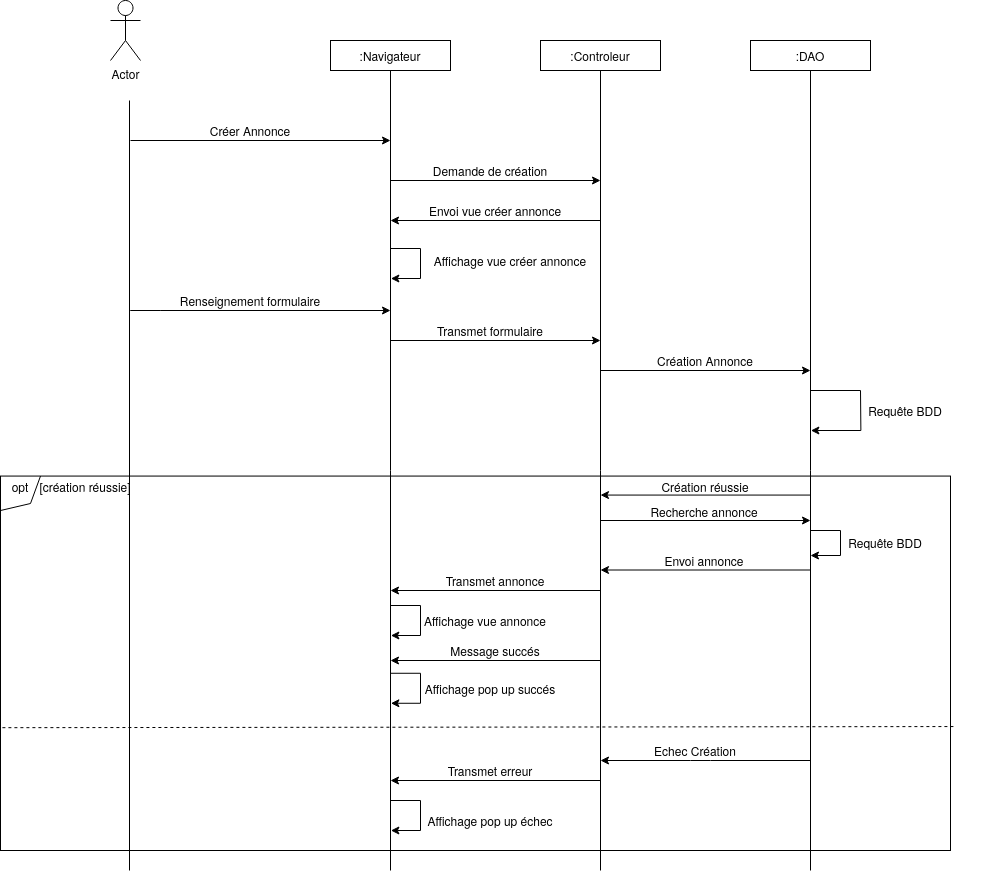
\includegraphics[width=350px]{../Conception/DS_annonce.png}
  \caption{Diagramme de Séquence haut niveau représentant la création d'une annonce}
  \label{fig:<un-label-court>}
\end{figure}

\paragraph{Diagramme de classes}\mbox{} \\

Pour faire le lien entre la base de données et les contrôleurs, on utilise plusieurs classes PHP comme définies par le diagramme de classes ci-dessous,
plus la classe DAO qui permet l'accès à la base de données (cette dernière n'apparaît pas pour des questions de visibilité) :\\

\begin{figure}[H]
  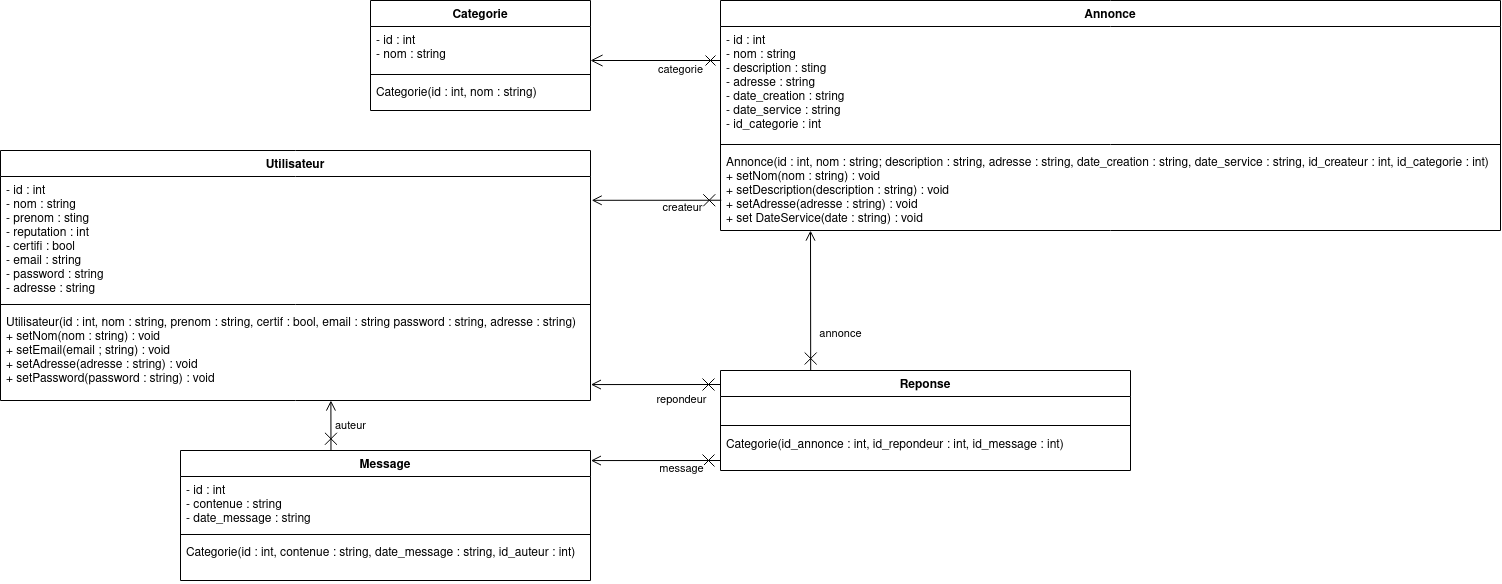
\includegraphics[width=\linewidth]{../Conception/PHP/DC.png}
  \caption{Diagramme de classes PHP}
  \label{fig:<un-label-court>}
\end{figure}

Pour la même raison, les \textit{getters} et \textit{setters} n'apparaissent pas, mais il y en a un pour chaque attribut.
L'attribut \texttt{Date\_creation} sert à indiquer la date de création de l'annonce.
En revanche, l'attribut \texttt{Date\_service} est optionnel dans le constructeur et sert à indiquer si l'annonce à un impératif de date.
Par exemple, pour de la garde d'enfants, la plupart du temps cela s'effectue sur un jour précis si ce n'est pas hebdomadaire.\\

\subsubsection{Conception base de données}

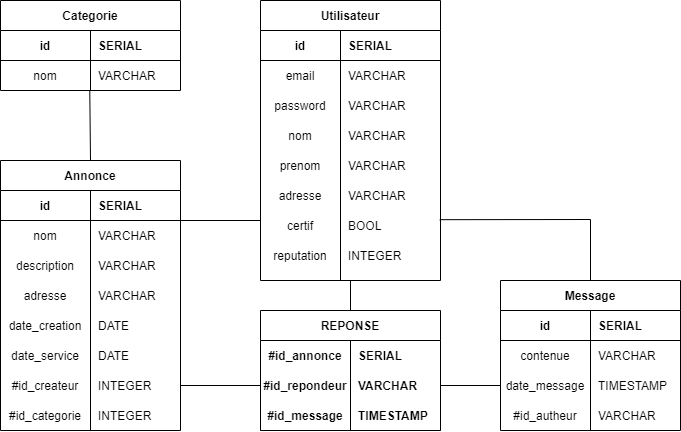
\includegraphics[width=400px]{images/Schema-relationnel-BDD.png}\\\\
SERIAL est un type de données fourni par PostgreSQL qui sert à créer des ID, il est équivalent à un entier qui s'auto-incrémente par défaut à chaque INSERT.\\\\
\textbf{Utilisateur(\underline{id}, email, password, nom, prenom, adresse, certif, reputation)}\\\\
\textbf{Categorie(\underline{id}, nom)}\\\\
\textbf{Annonce(\underline{id}, nom, description, adresse, date\_creation, date\_service, \#id\_createur, \#id\_categorie)}\\
id\_createur clé étrangère de Utilisateur.\\
id\_categorie clé étrangère de Categorie.\\\\
\textbf{Message(\underline{id}, contenue, date\_message, \#id\_auteur)}\\
id\_auteur clé étrangère de Utilisateur.\\\\
\textbf{Reponse(\underline{\#id\_annonce, \#id\_repondeur, \#id\_message})}\\
id\_annonce clé étrangère de Annonce.\\
id\_repondeur clé étrangère de Utilisateur.\\
id\_message clé étrangère de Message.\\\\
\textbf{Certificateur(\underline{id}, email, password, nom, prenom)}\\

Lorsqu'un utilisateur choisit une annonce qu'il a créée, on lui affiche la liste de personnes ayant répondu. Après son choix, il nous reste alors tous les messages entre le créateur de l'annonce et le répondeur.


\subsection{Solutions techniques envisageables}

Compte tenu des besoins détaillés précédemment, le service que nous souhaitons mettre en œuvre
sera réalisé par un service Web, et non par une application logicielle à installer qui serait moins
adaptée au public cible. La conception d’un site Web dynamique se décompose en : \\

\begin{itemize}
  \item Une IHM qui s’exécute sur le navigateur client avec la gestion locale des animations, formulaires, ...
  \item Une logique applicative qui s’exécute sur un serveur distant protégé afin de garantir la protection
  des données des utilisateurs et gérer l’accès et le stockage persistant des données.
  \item Une communication entre client et serveur qui utilise des protocoles standards sécurisés HTTPS.
\end{itemize}


Pour implémenter la partie IHM, les solutions envisageables sont basées sur les différentes
technologies actuelles.
L’ossature des pages sera en HTML et en CSS pour gérer la charte graphique, la structure des
bandeaux et des centres de page. On utilisera plus particulièrement la dernière version (HTML 5) qui permet
d’ajouter plus facilement des composants multimédia. Afin d’ajouter une dynamique moderne aux
pages (menu illustré par exemple) les sites Web actuels utilisent également des \textit{frameworks} Javascript
comme jQuery, AngularJS, ou React. Aux vues des délais et de la complexité des différent \textit{frameworks},
il est envisagé de n’utiliser que du HTML 5.\\

Pour implémenter la partie logique applicative et connexion aux stockages de données, qui doit être
sur un serveur distant sécurisé, il existe plusieurs technologies disponibles. On peut utiliser du PHP sur
serveur Apache ou NginX pour s’interfacer avec des fichiers ou des bases de données. Il est aussi possible de
recourir à l’usage de conteneurs JEE comme Tomcat, ou des serveurs d’application comme Weblogic
ou JBOSS. L’usage de Java JEE offre plus de possibilités, mais du fait de l’intensité du travail demandé
pour le développement et la complexité associé à JEE, il est préférable de baser notre service sur PHP.
Il est envisagé d'utiliser un serveur NginX car celui-ci et plus récent, gère mieux les connexions
multiples et a une configuration plus simple qu'Apache.\\

Pour implémenter le stockage de l’information, il existe plusieurs possibilités : le stockage dans des
fichiers, ou bien l’utilisation d'une base de données, qu’elle soit non relationnelle comme MongoDB,
Cassandra, ou relationnelle comme PostgreSQL, Oracle DB, MySQL ou bien SQLite. Compte tenu des
informations à stocker et des possibilités de recherche offertes sur l’IHM, une base de données et un
modèle relationnel sont plus indiqués. En effet les données que l'on manipule sont catégorisables
en n-uplets ordonnés (les données de profil d'un utilisateur, les données d'une annonce, etc), la
cardinalité entre ces relations est facilement définissable (un utilisateur a plusieurs anonces, les
annonces ont des types communs, des lieux ...) et les capacités de manipulation des données que l'on
veut proposer s'appuient simplement sur une combinaison de ces relations. De plus, un tel modèle permet de
limiter la duplication des données. Ce type de relations et de schémas d'accès sont caractéristiques
d'un modèle relationnel. Compte tenu du temps imparti et de nos connaissances,
il est envisagé d’utiliser une base relationnelle simple et facilement intégrable avec PHP et
dans un serveur NginX, comme PostgreSQL.\\
\pagebreak

Pour sécuriser l’accès aux services du site, il est nécessaire de mettre un place une authentification
avec un accès en mode HTTPS pour protéger les données qui circuleront sur le réseau. Il existe
plusieurs protocoles possibles pour l’authentification, notamment pour le SSO (Single Sign-On) comme SAML ou
OAUTH2 avec certificats ou identifiant et mot de passe. Il est aussi possible de déléguer l'authentification
SSO à des grandes entreprises du numérique comme Google ou Facebook, qui mettent à disposition des développeurs leur \textit{framework} d'authentification.
Ce type d'authentification qui permet de limiter la création des comptes est appelé Social Login.
Dans notre cas, le but est de permettre aux personnes âgées de ne pas avoir à s’inquiéter de retenir un mot
de passe et ainsi faciliter l’utilisation de notre site. Si le temps le permet, nous ajouterons le Social Login
via Google, mais en raison de l’échéance, l’authentification se fera dans un premier temps de façon classique, à
travers un simple identifiant (l'email) + mot de passe sur HTTPS. Les informations d’identification seront stockées
dans une partie spécifique de la base de données. Cette dernière stockera aussi les préférences des utilisateurs. \\

Le tableau ci-dessous résume les possibilités pour chaque catégorie et montre (cases bleues)
les choix que nous avons fait pour le projet \\

\begin{figure}[H]
  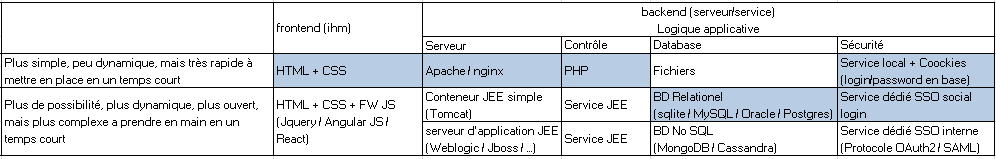
\includegraphics[width=\linewidth]{images/choixTechno.PNG}
  \caption{Choix technologiques pour le projet}
  \label{fig:choix-techno}
\end{figure}

\subsection{Réalisations techniques}

Compte tenu des choix techniques faits pour la réalisation (HTML/CSS, NginX, PHP, PostgreSQL) nous avons
mis en place un serveur NginX avec son module PHP et un \textit{driver} Postgres. Le tout a été déployé
sur un serveur Linux.\\

Pour le développement nous utiliserons des éditeurs de code standard (Atom, Visual Studio Code, Vim), et Visual Paradigm
pour le design des images et composants graphiques.\\

Le partage du code, le stockage et la gestion des versions seront gérés par un dépôt Git hébergé sur
Gricad-GitLab.\\

Pour faciliter la mise en place d'un environnement de travail, nous avons créé une machine virtuelle
reproduisant l'environnement du serveur de production (serveur web et base de données) et comprenant
aussi tous les outils nécessaires au développement (éditeur de texte + git). Ainsi les développeurs
ont juste à lancer la machine virtuelle et peuvent directement commencer à coder et tester leur code.

\subsection{Organisation du travail}

\subsubsection{Choix du modèle}

Pour ce projet, nous utiliserons une méthode itérative. Nous effectuerons des itérations toutes les 4
à 5 semaines de travail. Avec cette méthode, la mise en commun et l'intégration au sein du groupe se font toutes les semaines.
Cela permet de corriger au plus tôt les problèmes liés au partage des tâches et les potentiels retards.\\

\subsubsection{Découpage du projet}

Pour la deuxième itération, le projet a été découpé en 3 parties. L’équipe sera divisée en 3 binômes.\\

Ce choix de binôme permet une plus grande flexibilité et une parallélisation des tâches, tout en étant
moins stressant que du travail seul.\\

Sur ce diagramme, Alexandre et Lucas s'occuperont du visuel du site,
Elian et Marion s'occuperont de la logique de fonctionnement et
Eliott et Vincenzo s'occuperont du stockage des données.\\

\begin{figure}[H]
  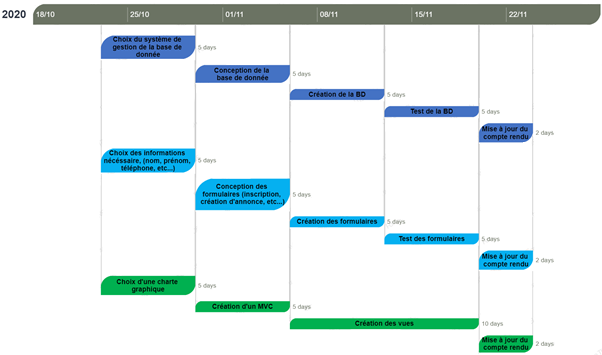
\includegraphics[width=\linewidth]{images/gantt-iteration2.png}
  \caption{Diagramme de GANTT pour l'Itération 2}
  \label{fig:gantt-iteration2}
\end{figure}

Suite à cette itération, les trois équipes on pris du retard, le travail était trop conséquent pour le temps donné.\\
En effet, tous les binômes ont du retard. L'équipe stockage des données a une semaine de retard.
L'équipe logique de fonctionnement a dû sauter quelques formulaires, le retard est d'environ une semaine.
Et l'équipe visuels n'a pas eu le temps de faire toutes les vues prévues, le retard est de deux semaines, car leur binôme était celui avec le plus de travail.

\begin{figure}[H]
  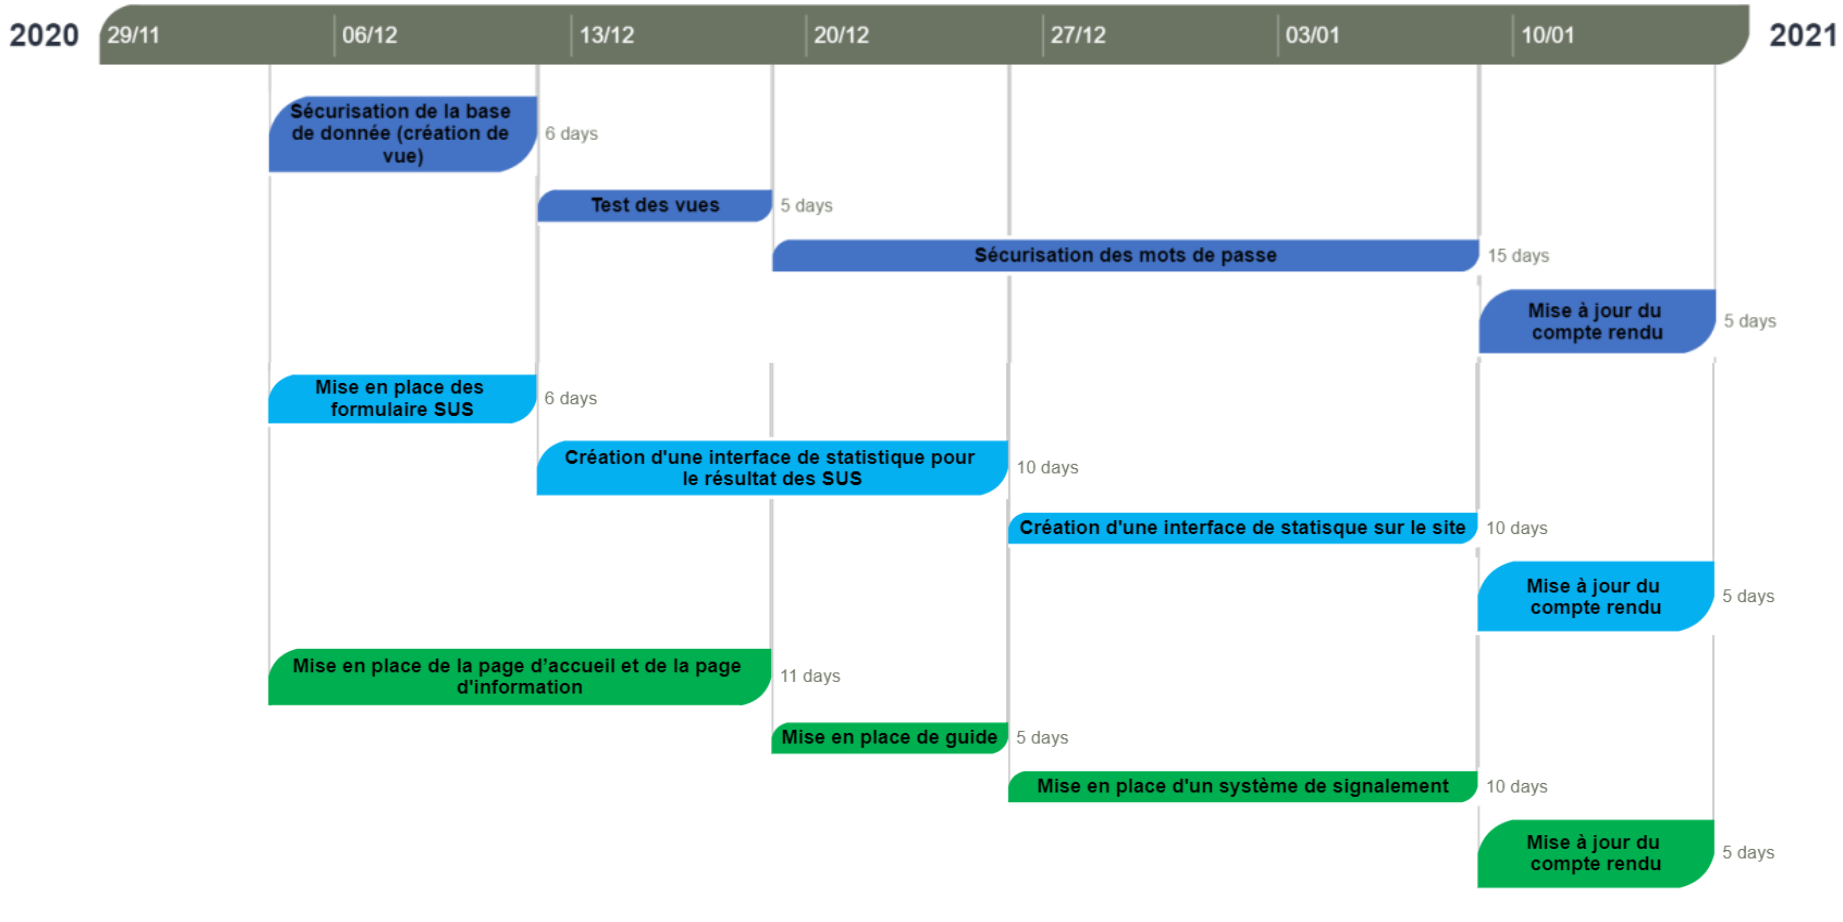
\includegraphics[width=\linewidth]{images/gantt-iteration3.png}
  \caption{Diagramme de GANTT pour l'Itération 3}
  \label{fig:gantt-iteration3}
\end{figure}


%===============================================================
%                           AVANCEMENT
%===============================================================

\section{Avancement du projet}

À l'heure actuelle, un serveur est déployé sur un Raspberry Pi, et l'infrastructure et le modèle MVC
avec base de données sont fonctionnels. Nous avons donc un programme PHP qui va chercher les
données du modèle dans une base de données PostgreSQL pour produire un affichage de pages
dynamiques avec du HTML/CSS grâce à un serveur Web NginX.\\


% ---------- Annonces ----------

\subsection{Annonces}

La fonctionnalité principale du service, à savoir la gestion d'annonces, est opérationnelle.\\

Les utilisateurs connectés peuvent créer une annonce depuis le bouton "Créer une annonce" accessible n'importe où sur le site ; on leur demande alors de rentrer les informations relatives à leur annonce (titre, description, etc...) et leur annonce est enregistrée dans la base de donnée. Ces utilisateurs peuvent ensuite accéder aux annonces qu'ils ont déja créées depuis la page de leur profil.\\

Une page "Rechercher une annonce" affiche les annonces, récupérées dynamiquement depuis la base de données, sous forme d'aperçus (titre, catégorie, début de description) ; elle permet également de les filtrer par catégorie, ou de rechercher par mots-clés (pour l'instant assez sommaire).\\

Chaque aperçu d'annonce permet d'accéder à une page présentant plus en détails l'annonce en question.\\
Depuis cette page, le créateur de l'annonce peut la modifier ou la supprimer ; les autres utilisateurs peuvent répondre à l'annonce (voir section "Messages") ou la signaler si elle est inapropriée.\\

\subsection{Messages}

Les utilisateurs peuvent interagir via le système de messages. Un utilisateur intéressé par une annonce peut y répondre, ce qui crée un fil de discussion lié à cette annonce et à son auteur, pour permettre aux deux parties de se mettre d'accord. Chaque utilisateur, via son profil, a accès à toutes ses conversations, que ce soit pour ses propres annonces ou pour celles auxquelles il a répondu. Enfin, si l'auteur d'une annonce juge que l'accord est conclu après une réponse, il peut la marquer comme "Validée", ce qui retire l'annonce des pages de recherche et envoie un message automatique à son interlocuteur.

% ----------Compte ----------

\subsection{Compte}

La création de compte est maintenant disponible via une page dédiée \textit{(Capture d'écran en annexe)}. Un avertissement en cas de non-remplissage de certain champs ou de mauvais remplissage (comme un format d'adresse mail invalide) facilite l'utilisation du formulaire.\\
Une fois le compte créé et l'utilisateur connecté, il a accès à sa page de profil, d'où il peut consulter ses annonces et ses conversations, modifier ses informations personnelles et supprimer son compte.


% ---------- Certification des utilisateurs ----------

\subsection{Certification des utilisateurs}

La priorité parmi les différents types de certification a été la certification d'identité par un tiers. Un utilisateur certifié est reconnaissable par un badge vert à côté de son nom.\\

Le système de réputation, étant secondaire, n'a été implanté que partiellement et n'est pas fonctionnel à l'heure actuelle. Cependant, il reste dans notre liste de priorité si nous voulons achever le site entièrement.


% ---------- Type de compte ----------

\subsection{Type de compte}

Actuellement, les deux types de compte existants sont les comptes utilisateurs et les comptes certificateurs. Les comptes utilisateurs sont créés via la page d'inscription et correspondent à un utilisateur standard, alors que les comptes certificateurs sont gérés par une autorité de certification des utilisateurs tels qu'une mairie ou une association, et sont créés directement en base de données pour l'instant. Cette pratique peut poser des problèmes tels qu'une mauvaise saisie ou une erreur de requête SQL. C'est pour cela que, à terme, nous ferons un compte "administrateur" avec la possibilité de créer des comptes certificateurs et des capacités de modération telles que le bannissement temporaire ou permanent de membres.
Si l'affluence du site devient importante, nous devrons créer des comptes modérateurs pour gérer les éventuels abus.\\

Nous avons donc contacté une mairie pour savoir si elle était intéressée et nous avons reçu une réponse plutôt positive. Ils sont prêts à accepter de certifier l'identité des utilisateurs à conditions que nous soyons capables de prouver que notre site est apte à contenir des informations sensibles et respecte la RGPD. Pour l'instant, notre site n'étant pas assez abouti, ils n'ont pas voulu s'investir sur le plan humain et financier.

% ---------- Localisation ----------
\subsection{Recherche par localisation}
La recherche par localisation avait été identifiée comme un besoin fonctionnel,
mais ayant une priorité assez basse par rapport aux autres fonctionnalités, nous n'avons
pas eu le temps de la réaliser. L'utilisateur peut tout de même rechercher des annonces par mot-clé
et catégorie, mais ne peut actuellement spécifier une zone géographique.

% ---------- secutite ----------
\subsection{Sécurité}
Notre site étant en phase de prototype, la sécurité n'est pas maximale. Notamment au niveau de la gestion de mot de passe qui est, pour l'instant, entrée en clair dans la base de donnée. L'une des solutions est de hacher les mots de passe avant chaque accès en base (pour les entrer ou les comparer) pour que même s'il y a une fuite de sécurité, l'impact soit limité. Cependant, pour maintenir l'intégrité du site, certaines failles ont été corrigées comme les injections de code ou encore le protocole qui a été passé en http.

% ---------- Guidage ----------
\subsection{Guidage}
\subsubsection*{Erreurs}
Pour améliorer la prévention des erreurs, nous avons mis en place différents mécanismes:
\begin{itemize}
  \item Un message de confimation en pop-up apparaît lorsque l'utilisateur s'apprête à réaliser une action critique, comme supprimer une annonce/son compte.
  \item Lors de la création d'une annonce, si l'utilisateur entre une date antérieure à la date actuelle, un message d'erreur l'empêche de créer l'annonce.
\end{itemize}

De même pour la gestion des erreurs:
\begin{itemize}
  \item Après avoir créé une annonce/un compte, l'utiliseur peut toujours le modifier s'il se rend compte d'une erreur.
  \item Si jamais une erreur survient (404 etc..), une page personnalisée est prévue à cet effet, permettant à l'utilisateur de revenir sur le site.
\end{itemize}

% ---------- Évaluation ----------

\subsection{Évaluation du site}

Pour pouvoir tester et évaluer notre site, nous l'avons fait tester à des membres de notre famille, à des amis, en bref, à la plus grande diversité de profils de personne. Pour avoir une continuité et stabilité dans l'évaluation, nous nous sommes basées sur les critères ergonomiques de Bastien et Scapin pour notre grille d'évaluation. Elle comprend donc : le guidage, le contrôle explicite, la gestion d'erreur, la charge de travail et l'homogénéité. Cependant, en ce qui concerne l'adaptabilité, nous avons décidé de ne pas en tenir rigueur pour garder une simplicité optimale. Nous n'avons pas non plus tenu rigueur de la compatibilité, car, visant un public de tout horizon, les habitudes et caractéristique de chacun sont aussi nombreuse que varier. Il est donc difficile d'évaluer ce critère. En ce qui concerne les autres éléments, nous avons demandé aux testeurs d'attribuer une note sur dix par catégorie.\\
Cela nous donne une moyenne générale de 8.52/10 avec :\\
\begin{itemize}
  \item Guidage : 8.3/10
  \item Contrôle explicite : 7/10
  \item Gestion d'errur : 8.5/10
  \item Charge de travail : 8.75/10
  \item Signifiance des codes et dénominations : 9.3/10
  \item Homogeneité : 9.25/10
\end{itemize}

Nous avons aussi rédigé un petit scénario à suivre lors de l'évaluation telle que :
\begin{enumerate}
  \item Rechercher une annonce existante en base
  \item Tenter d'y repondre (ce qui est impossible sans être connecté)
  \item Crée un compte
  \item Répondre a l'annonce rechercher plutôt
  \item Crée une annonce
  \item La modifier
  \item Modifier son compte (crée plutôt)
  \item Supprimer son compte
  \item Signaler une annonce
\end{enumerate}

Le détail des notes et profile pour chaque personne se trouve en annexe.

% ---------- Utilisation (pour les profs) ----------

\subsection{Utilisation}

Pour faciliter le test aux enseignants, nous avons créé des comptes avec des éléments pré remplie comme une annonce, quelques réponses, etc...\\

Les identifiant des comptes utilisateurs sont pour le login "prenom.nom@iut2.univ-grenoble-alpes.fr" et le mot de passe est "ens"

Nous avons aussi créé un compte certificateur unique avec pour login "ens@iut2.univ-grenoble-alpes.fr" et comme mot de passe ens.\\

Cependant, cela n'empêche en rien de test la création de compte, d'annonce ou quelques fonctionnalités que ce soit.

Le lien du site : https://art-entraide.ddns.net:8080


\newpage


%===============================================================
%                           ANNEXE
%===============================================================


\section{Annexe}

\subsection{Analyse de l'existant}

\subsubsection{Services}

Notre projet consistant à fournir un service, il nous fallait regarder quels sont nos concurrents sur le marché.
Visent-ils une rentabilité ou simplement à rendre service ? Pour cela, nous avons vérifié si, pour chaque site,
il était possible de rendre un service gratuitement, contre un autre service ou en étant payé.\\

AlloVoisins possède des services gratuits (dits “non-rémunérés”) mais ils sont très peu utilisés,
dû au fait qu’il est impossible d’échanger ce service contre un autre.\\

\begin{figure}[H]
  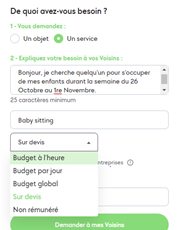
\includegraphics[width=200px]{images/services-allovoisins.png}
  \label{fig:services-allovoisins}
\end{figure}

Pwiic propose un système d’échange de pièces contre des services. Ces pièces peuvent être soit achetées,
soit gagnées en échange des services. Le site se base sur une proposition de prix, plutôt qu’un prix fixé au départ.\\

\begin{figure}[H]
  
\includegraphics[width=250px]{images/pieces-pwiic.png}
  \label{fig:pieces-pwiic}
\end{figure}

YakaSaider met en place des profils : par exemple, ici, Aurélie est coiffeuse. Il n’y a aucun prix affiché,
aucune durée, juste un bouton "Contacter". Sur ce site, il faut payer en heures. Lorsque l’on crée un compte,
on dispose d’une heure "gratuite" après quoi il faut rendre des services pour en gagner.
On les consomme lorsque l’on demande un service.\\

\begin{figure}[H]
  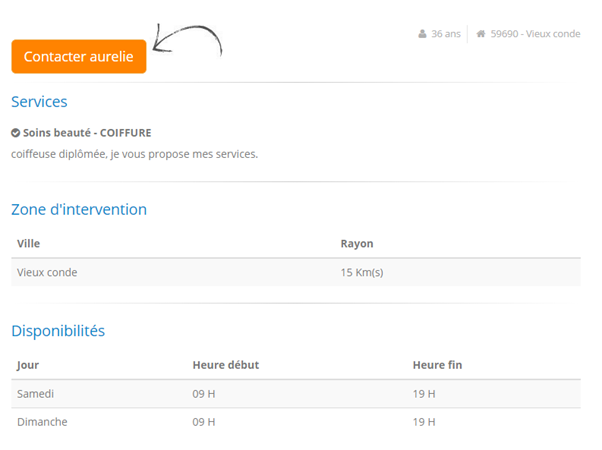
\includegraphics[width=500px]{images/aurelie-yakasaider.png}
  \label{fig:aurelie-yakasaider}
\end{figure}

\pagebreak

\subsubsection{Critères d'ergonomie}

Étant donné le public cible, il est important de respecter certains critères ergonomiques.\\

\paragraph{Guidage}

Nous nous sommes laissés guider sur les sites, pour voir comment ces sites s’y prenaient pour attirer
l’attention là où se trouve l’information.\\

AlloVoisins a un guidage simple. Les boutons importants sont en couleur.\\

\begin{figure}[H]
  
\includegraphics[width=350px]{images/Guidage-allovoisins.png}
  \label{fig:Guidage-allovoisins}
\end{figure}

Mais pour les demandes, le titre de la demande est l’endroit où il faut cliquer pour accéder aux informations,
or il n’est pas assez mis en valeur.\\

\begin{figure}[H]
  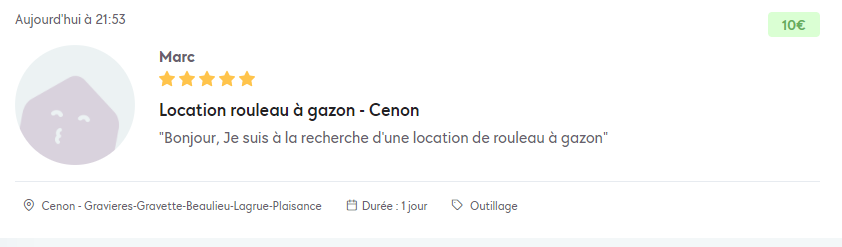
\includegraphics[width=350px]{images/demande-allovoisins.png}
  \label{fig:demande-allovoisins}
\end{figure}

Pwiic a un guidage peu intuitif. Par exemple, sur les cartes servant à donner les caractéristiques d’une personne
lorsque l’on cherche un service, le bouton "Voir ce Pwiic" n’est pas en couleur. De plus, le pouce en l’air donne
l’impression que le bouton est là pour donner un avis et non pour voir le profil.\\

\begin{figure}[H]
  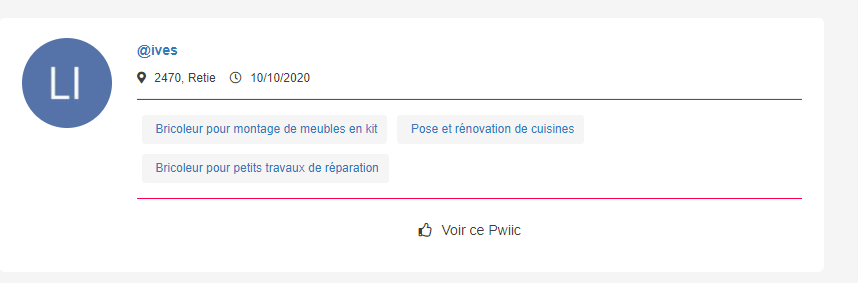
\includegraphics[width=350px]{images/guidage-pwiic.png}
  \label{fig:guidage-pwiic}
\end{figure}

Et lorsque l’on clique sur "Voir ce Pwiic", le bouton pour contacter la personne n’est pas trouvable du premier coup d’œil.\\

\begin{figure}[H]
  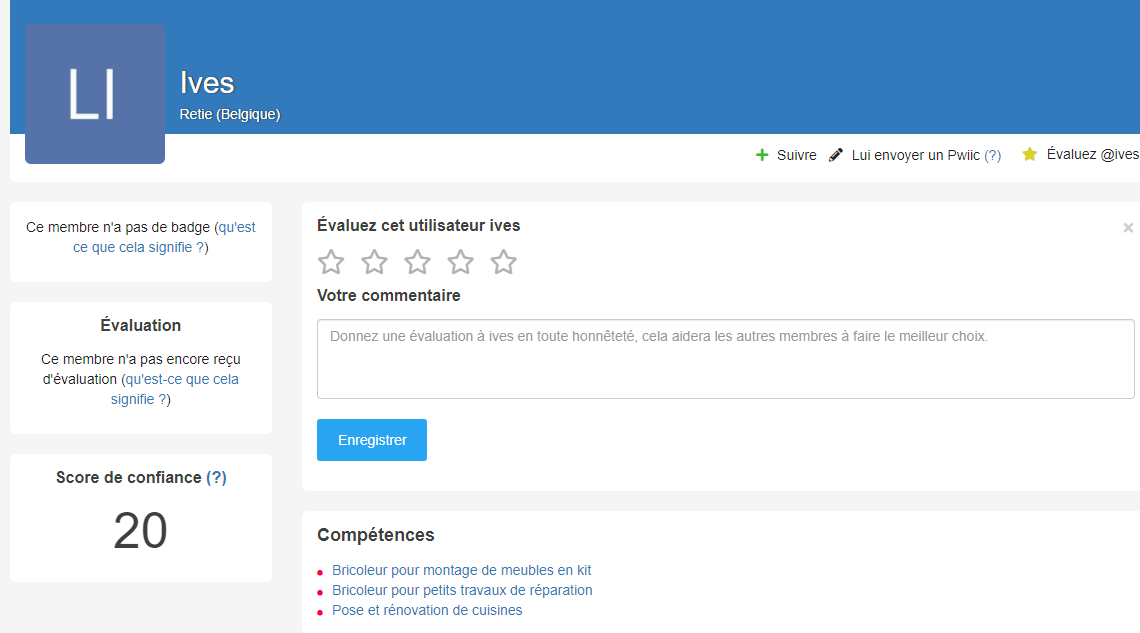
\includegraphics[width=350px]{images/voir-ce-pwiic.png}
  \label{fig:voir-ce-pwiic}
\end{figure}

De plus, le mot "Pwiic" est un terme abstrait créé à partir du nom de marque du site, moins clair que "annonce"
par exemple, ce qui ne facilite pas forcément la navigation pour des personnes peu à l’aise.

YakaSaider possède un guidage peu efficace. Lorsque l’on recherche pour "Tous les services", on ne voit aucune
compétence ni même description, seulement le visage de la personne, son nom et sa ville.\\

\begin{figure}[H]
  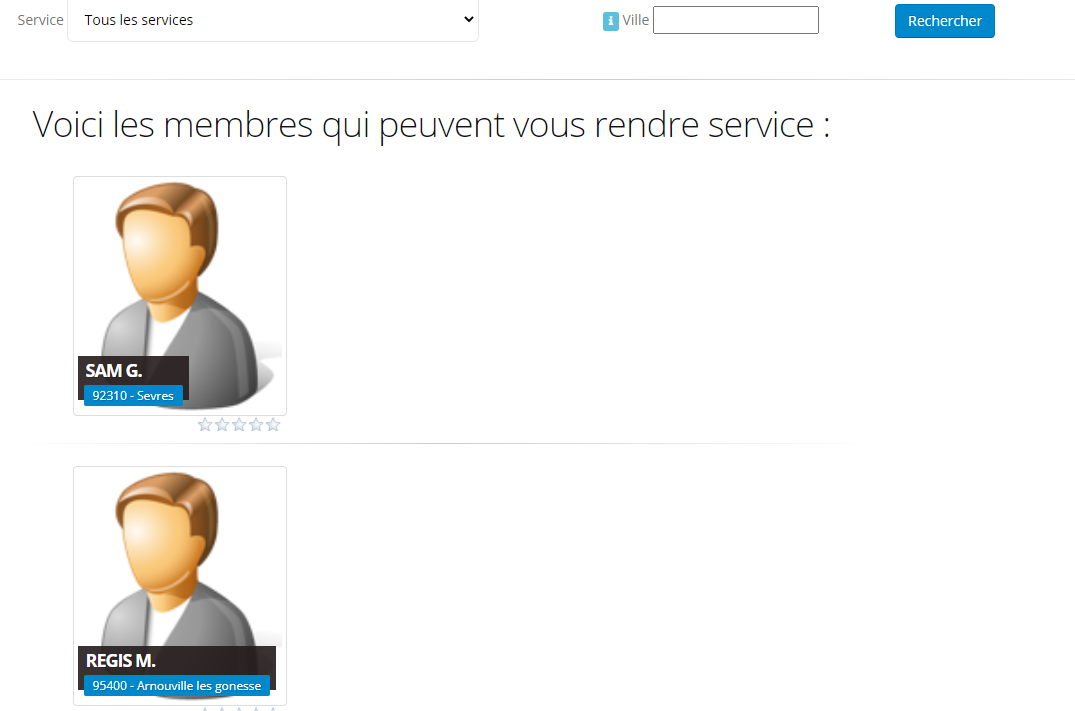
\includegraphics[width=400px]{images/guidage-yakasaider.png}
  \label{fig:guidage-yakasaider}
\end{figure}

Pour régler le problème, il faut faire une recherche plus affinée.\\

\paragraph{Gestion des erreurs}

Ensuite, nous avons essayé de faire des actions qui n’étaient pas celles demandées -- une erreur peut très vite perdre un utilisateur.\\

AlloVoisins et Pwiic semblent bien gérer les erreurs. Par exemple, si l’on saisit dans la barre de recherche quelque chose
qui n’est pas valable, on est renvoyé sur la page de résultats par défaut, c’est à dire tous les résultats près de
chez nous ou de l’endroit où notre demande se trouve.\\

\begin{figure}[H]
  
\includegraphics[width=\linewidth]{images/gestion-erreur-allovoisins.png}
  \label{fig:gestion-erreur-allovoisins}
\end{figure}

\begin{figure}[H]
  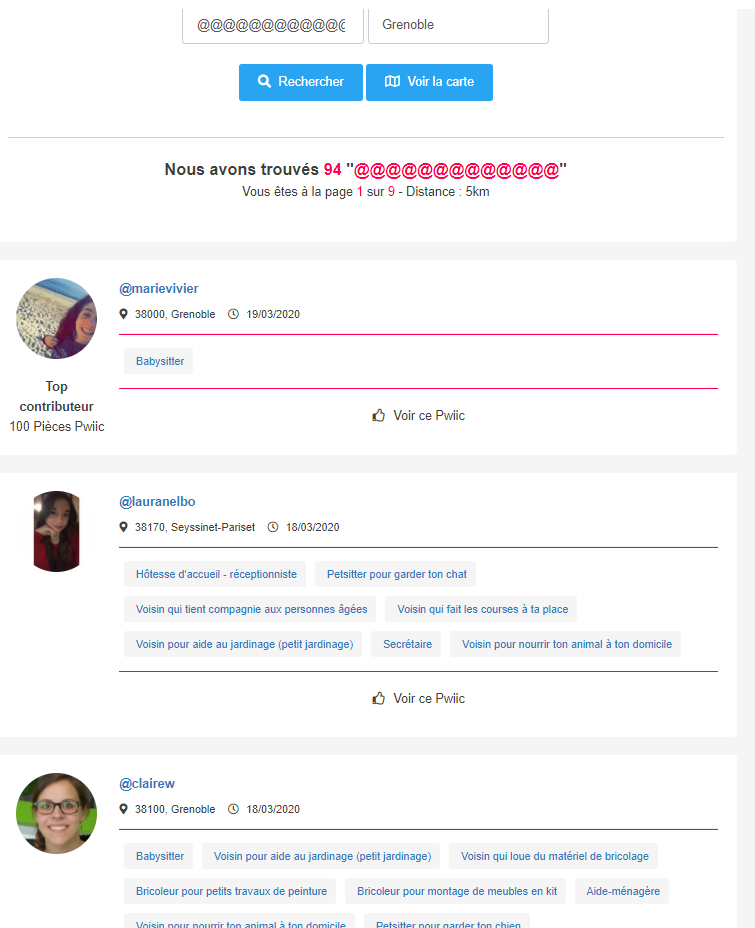
\includegraphics[width=350px]{images/gestion-erreur-yakasaider.png}
  \label{fig:gestion-erreur-yakasaider}
\end{figure}

YakaSaider gère le résultat de la recherche différemment. Lorsqu’aucun résultat n’est disponible,
il affiche simplement un message disant qu’aucun résultat n’a été trouvé.\\

\begin{figure}[H]
  
\includegraphics[width=\linewidth]{images/pas-trouve-yakasaider.png}
  \label{fig:pas-trouve-yakasaider}
\end{figure}

Mais la liste des services possède une erreur, on peut sélectionner les tirets qui servent à délimiter les catégories.\\

\begin{figure}[H]
  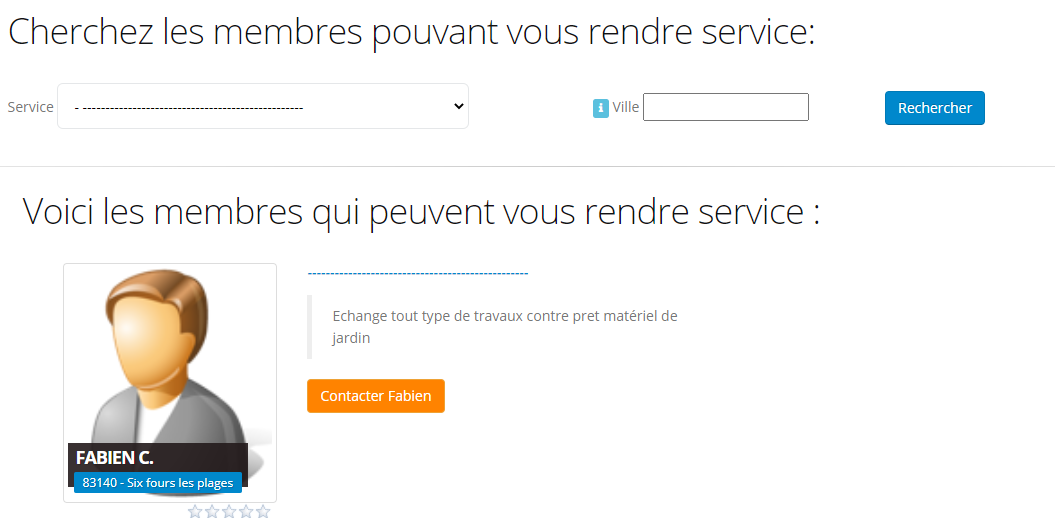
\includegraphics[width=\linewidth]{images/erreur-yakasaider.png}
  \label{fig:erreur-yakasaider}
\end{figure}

\paragraph{Certification}

Enfin, la certification nous semblait importante, puisqu’elle permet de limiter certains risques, tels que les arnaques.\\

YakaSaider et Pwiic ne possèdent aucun système de certification.\\

Pwiic ne demande même pas de nom, l’utilisateur s’identifie par un pseudo.\\

AlloVoisins possèdent un système où un utilisateur est certifié par son numéro de téléphone,
cela lui permet notamment d’accéder à la messagerie du site. (\href{https://support.allovoisins.com/hc/fr/articles/360000816614-Pourquoi-dois-je-certifier-mon-num%C3%A9ro-de-mobile-pour-pouvoir-acc%C3%A9der-%C3%A0-la-messagerie-}{source})

\subsection{Diragramme de séquence}

\begin{figure}[H]
  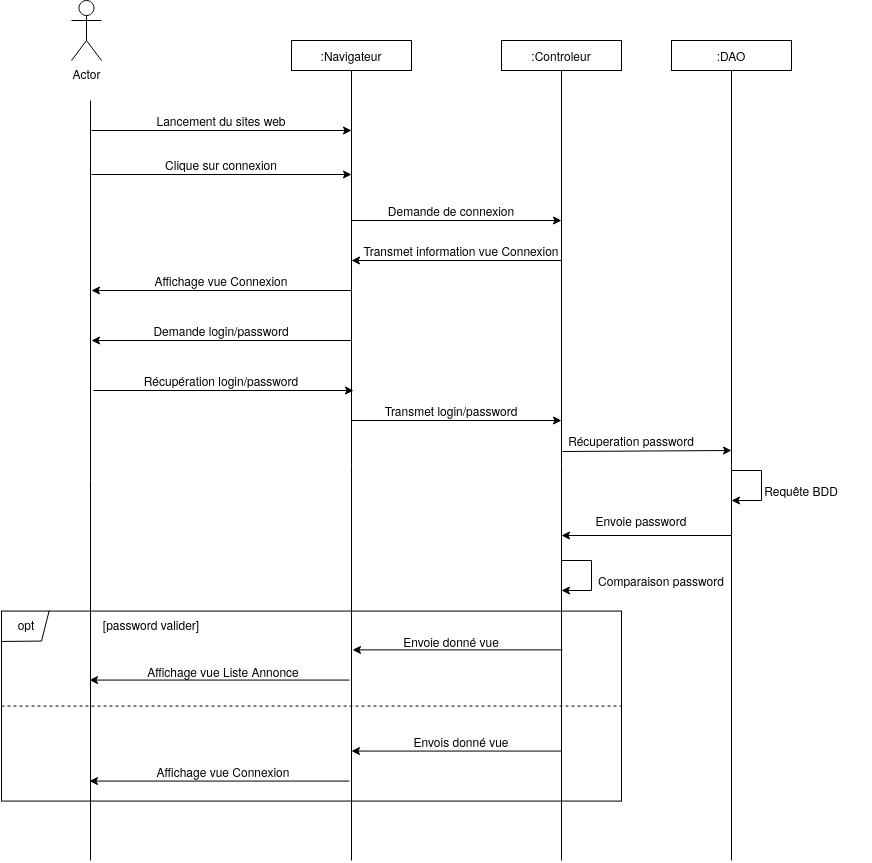
\includegraphics[width=\linewidth]{../Conception/DS_Connexion.png}
  \caption{Diagramme de Séquence haut niveau représentant l'authentification}
  \label{fig:ds-connexion}
\end{figure}

\subsection{Maquettes}
\label{sec:maquettes-annexe}

\subsubsection{Maquettes originales}

\begin{figure}[H]
  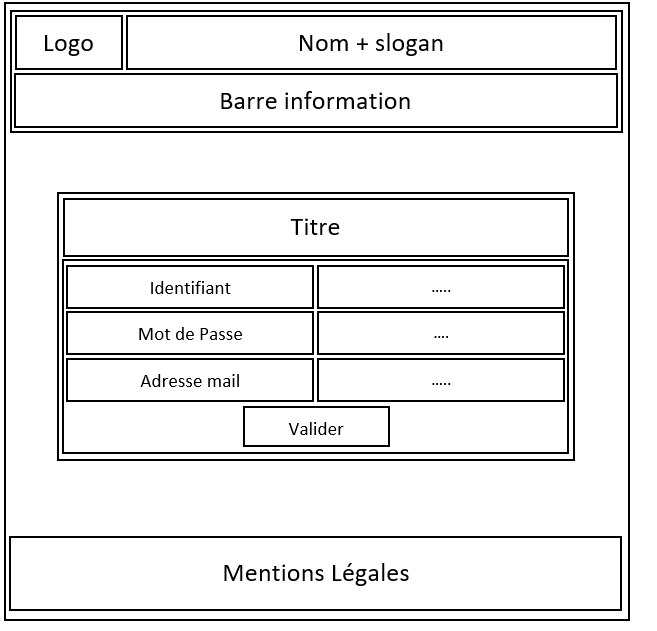
\includegraphics[width=\linewidth]{images/maquette-inscription-original.png}
  \caption{Maquette originale de l'inscription}
  \label{fig:maquette-inscription-original}
\end{figure}

\begin{figure}[H]
  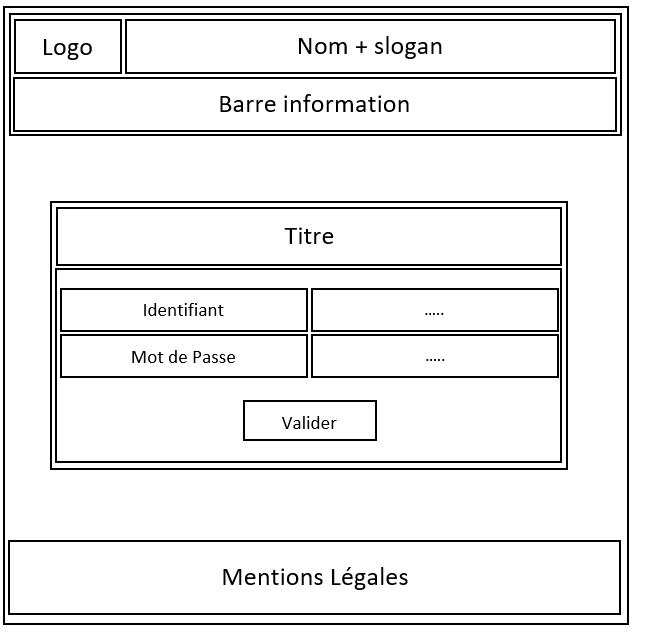
\includegraphics[width=\linewidth]{images/maquette-connexion-original.png}
  \caption{Maquette originale de la connexion}
  \label{fig:maquette-connexion-original}
\end{figure}

\begin{figure}[H]
  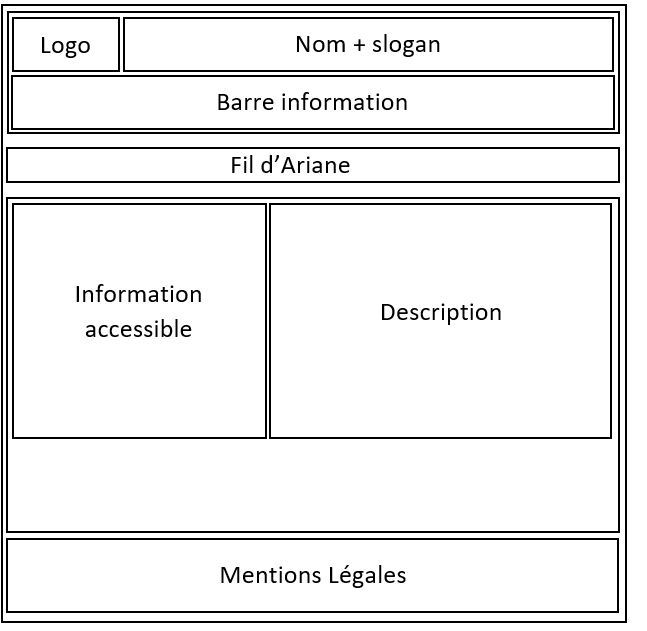
\includegraphics[width=\linewidth]{images/maquette-detail-annonce-original.png}
  \caption{Maquette originale du détail d'une annonce}
  \label{fig:maquette-detail-annonce-original}
\end{figure}

\begin{figure}[H]
  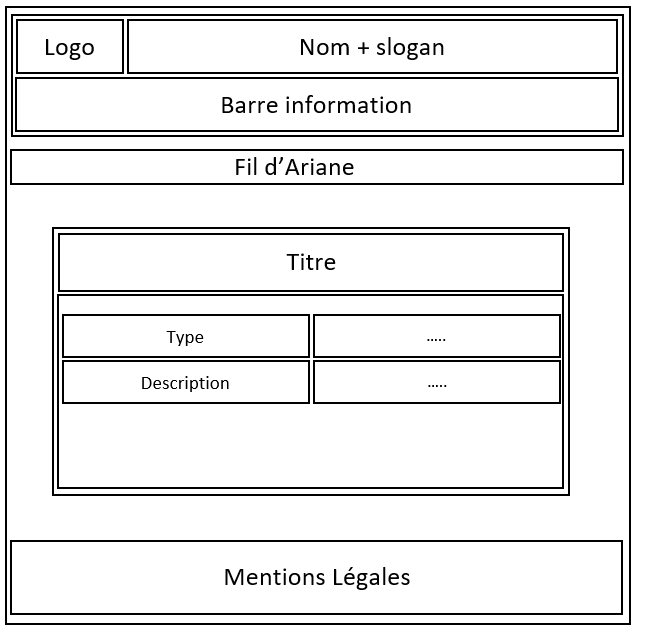
\includegraphics[width=\linewidth]{images/maquette-creation-annonce-original.png}
  \caption{Maquette originale de la création d'une annonce}
  \label{fig:maquette-creation-annonce-original}
\end{figure}
\newpage

\subsubsection{Maquettes actuelles}

\paragraph{Page du détail d'une annonce}

Pour appuyer sur le guidage, toutes les informations essentielles de l'annonce sont groupées sur la gauche.


\begin{figure}[H]
  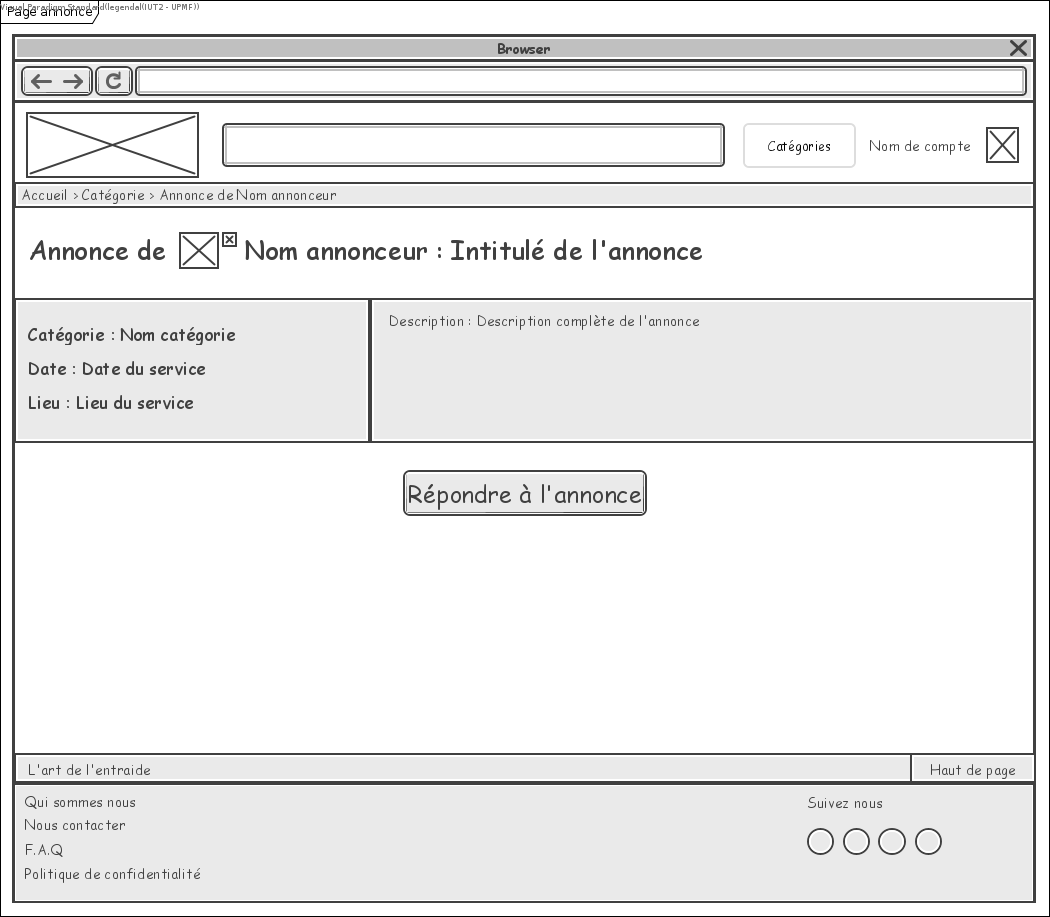
\includegraphics[width=\linewidth]{images/maquette-detail-annonce.png}
  \caption{Page du détail d'une annonce.}
  \label{fig:maquette-detail-annonce}
\end{figure}
\newpage

\paragraph{Page de création d'une annonce}

Sur cette page, nous avons essayé de réduire la densité informationnelle au maximum pour que publier
une annonce reste une action simple. Ainsi la page est constituée d'un titre, de 6 blocs, un pour chaque paramètre
de l'annonce, ainsi qu'un bouton pour confirmer.

\begin{figure}[H]
  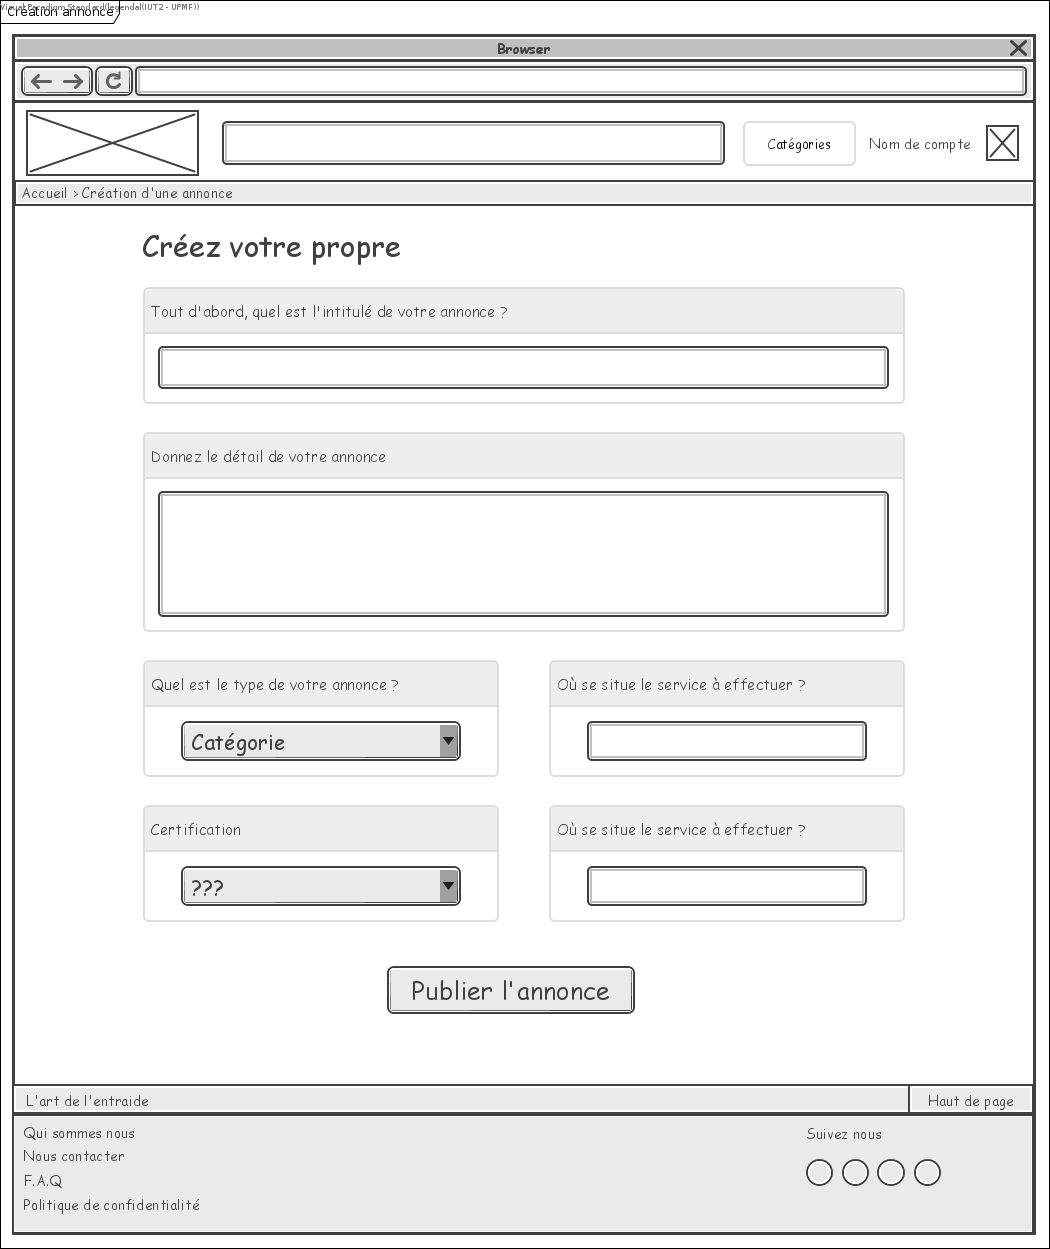
\includegraphics[width=\linewidth]{images/maquette-creation-annonce.png}
  \caption{Page de création d'une annonce.}
  \label{fig:maquette-creation-annonce}
\end{figure}
\newpage

\paragraph{Page d'inscription}

Sur la partie gauche de cette page, un paragraphe explique les avantages de créer son compte,
toujours dans l'objectif de renforcer le guidage. Sur la partie droite, un formulaire comportant
tous les champs nécessaires à la création de compte. La connexion via compte Google est aussi
disponible pour améliorer la brièveté, la flexibilité et la prise en compte de l'expérience de
l'utilisateur car cela rend l'inscription beaucoup plus accessible.

\begin{figure}[H]
  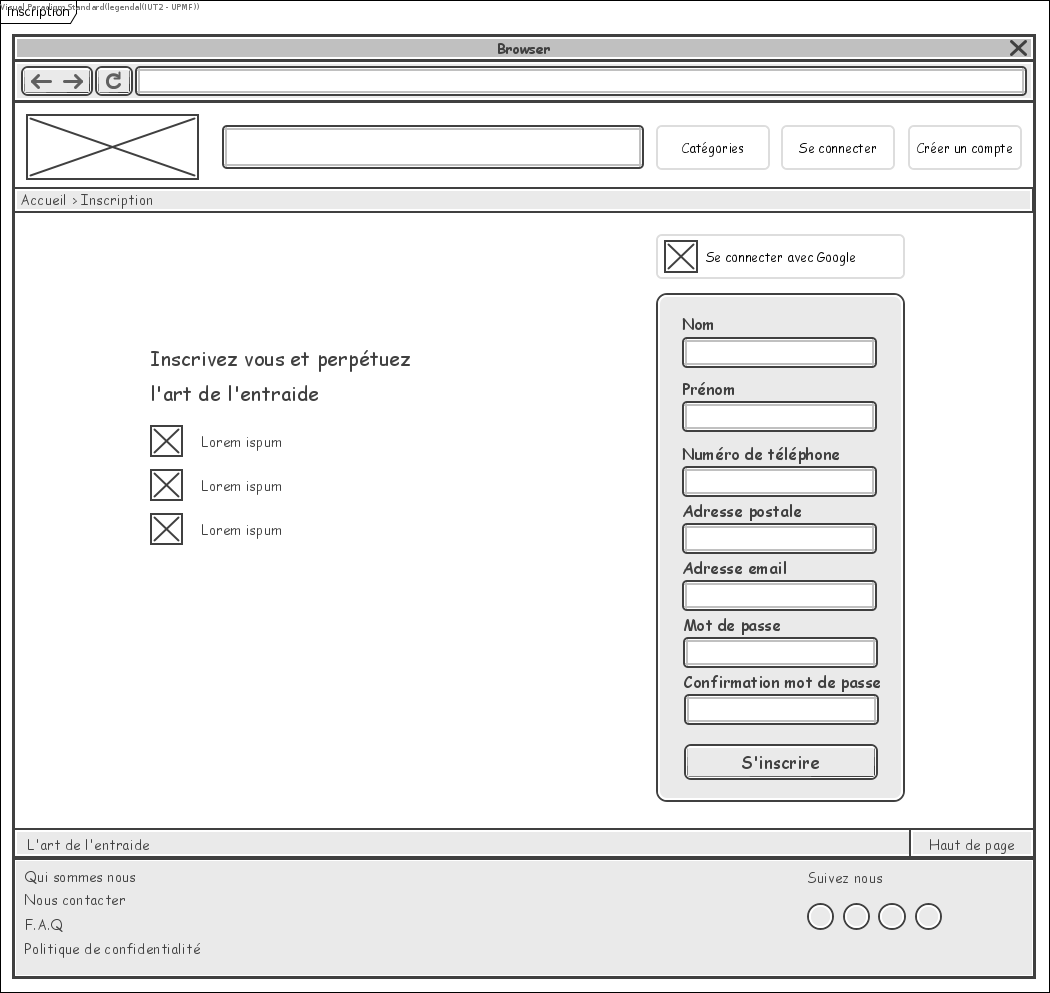
\includegraphics[width=\linewidth]{images/maquette-inscription.png}
  \caption{Page d'inscription.}
  \label{fig:maquette-inscription}
\end{figure}
\newpage

\paragraph{Page de connexion}

Cette page a pour but d'être simple, avec une densité informationnelle faible.
Un lien permet de rediriger vers la création d'un compte si l'utilisateur n'en
avait pas encore un, améliorant la correction des erreurs.
Encore une fois ici, la connexion via compte Google est présente pour plus de
flexibilité et de prise en compte de l'expérience de l'utilisateur.

\begin{figure}[H]
  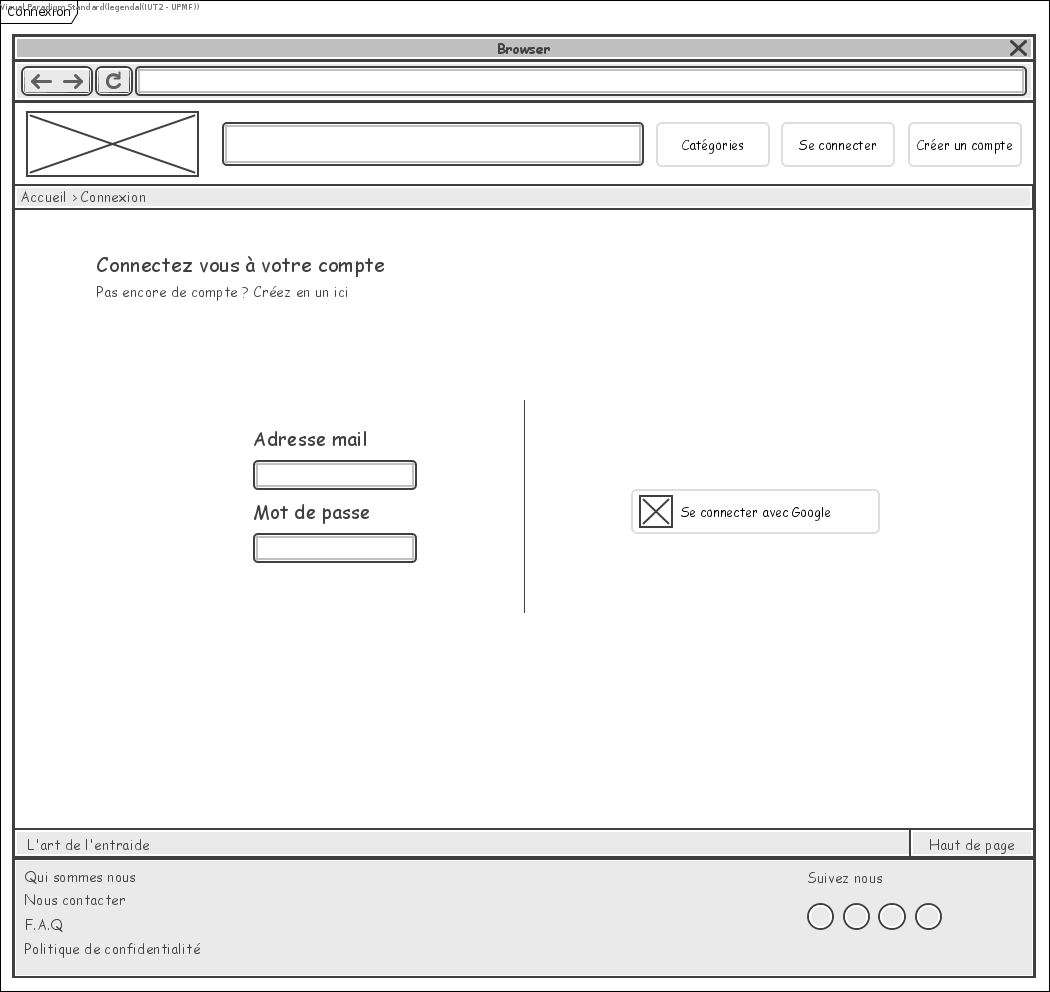
\includegraphics[width=\linewidth]{images/maquette-connexion.png}
  \caption{Page de connexion.}
  \label{fig:maquette-connexion}
\end{figure}
\newpage

\paragraph{Page de recherche d'annonce}

Sur cette page, les critères de recherches sont tous groupés sur une même ligne,
et la prévisualisation des annonces a été reprise de la page d'accueil pour plus de cohérence interne.

\begin{figure}[H]
  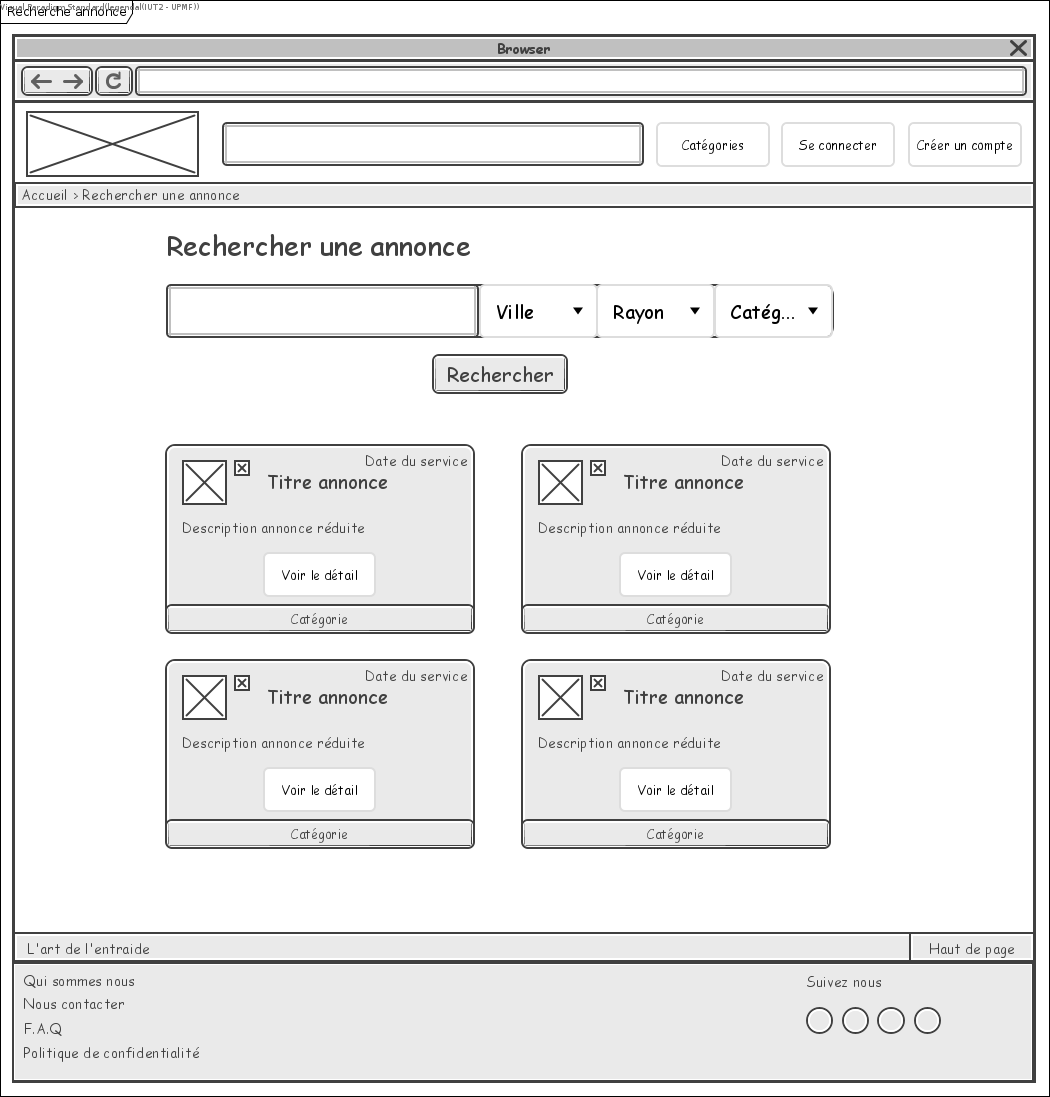
\includegraphics[width=\linewidth]{images/maquette-recherche.png}
  \caption{Page de recherche d'annonce.}
  \label{fig:maquette-recherche}
\end{figure}
\newpage

% ---------- screen inscription ----------

\subsection{Capture d'écran du site}


\subsubsection{Page d'inscription}

\begin{figure}[H]
  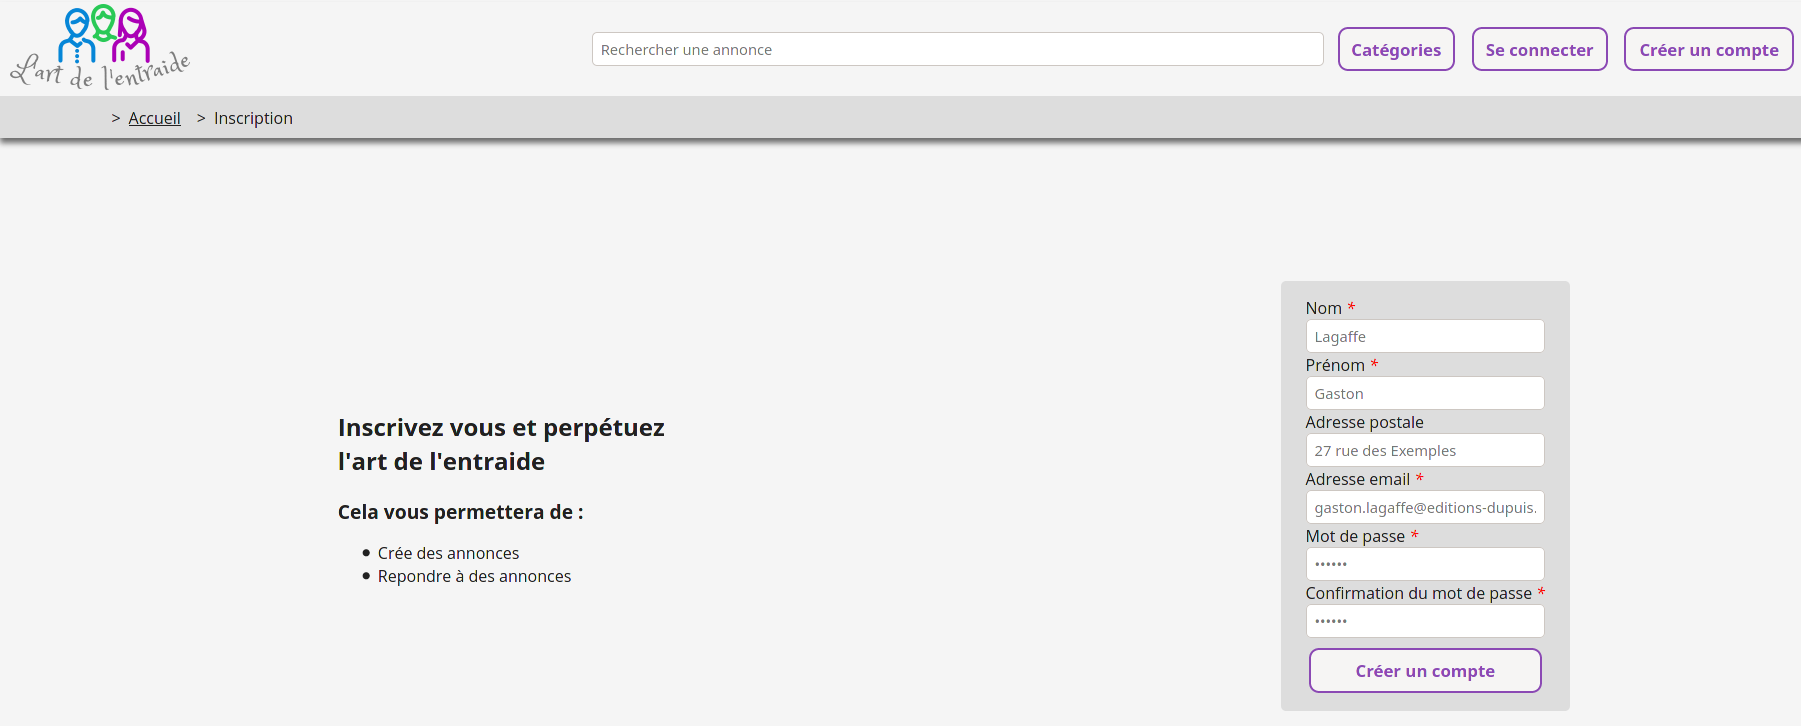
\includegraphics[width=\linewidth]{images/page-inscription.png}
  \caption{Page d'inscription.}
  \label{fig:page-inscription}
\end{figure}

\newpage

% ---------- Évaluation ----------

\subsection{Évaluation du site}

Toutes les personnes présentées ci-dessous ont donné leur autorisation d'apparaître ici avec les informations associées.
Les personnes qui ont testé et évalué le site sont :\\

Carole Pasini, 50 ans, secrétaire et plutôt à l'aise avec l'informatique.\\
Florian Attias, 19 ans, étudiant en biologie et à l'aise avec l'informatique.\\
Frederic Loraux, 49 ans, ouvrier et très très peu à l'aise avec l'informatique.\\
Sarah Loraux, 47 ans, secrétaire et plutôt à l'aise avec l'informatique.\\
Baptiste Guyard, 22 ans, étudiant.\\
Audrey Chauvineau, 22 ans, étudiante en nanotechnologie.\\
Laurent Chauvineau, 50 ans, ingénieur informaticient.\\
Mary-vonne et Pascal Prely, respectivement ingénieur et retraiter.\\
Xavier Sirvent, 51 ans, ingénieur informaticient.\\

\begin{center}
   \begin{tabular}{ | l | c | c | c | c | c | c | }

     \hline
     Profil & Guidage & \begin{tabular}[c]{@{}l@{}}Contrôle \\ explicite\end{tabular} & \begin{tabular}[c]{@{}l@{}}Gestion \\ des erreurs\end{tabular}  & \begin{tabular}[c]{@{}l@{}}Charge \\ de travail\end{tabular} & \begin{tabular}[c]{@{}l@{}}Signifiance des codes \\ et dénominations\end{tabular} & \begin{tabular}[c]{@{}l@{}}Homogénéité / \\ Cohérence\end{tabular} \\ \hline

     Carole Pasini      & 7,5/10 & 7/10       & 7/10   & 8/10    & 9/10       & 9/10    \\ \hline
     Florian attias     & 8,3/10 & 7/10       & 8/10   & 8/10    & non évalué & 8/10    \\ \hline
     Frederic Loraux    & 8/10   & non évalué & 9/10   & 9/10    & 9/10       & 10/10   \\ \hline
     Sarah Loraux       & 9.5/10 & non évalué & 10/10  & 10/10   & 10/10      & 10/10   \\ \hline
     Baptiste Guyard    & 8/10   & 9/10       & 10/10  & 9/10    & 8/10       & 8.6/10   \\ \hline
     Audrey Chauvineau  & 7.75/10& 8/10       & 8.3/10 & 9/10    & 9/10       & 9.5/10   \\ \hline
     Laurent Chauvineau & 10/10  & 10/10      & 9.3/10 & 8.5/10  & 10/10      & 10/10   \\ \hline
     Mary-vonne Prely   & 9.5/10 & 10/10      & 9/10   & 10/10   & 10/10      & 10/10   \\ \hline
     Xavier Sirvent     & 9.25/10 & 9/10      & 9/10  & 9.5/10  & 10/10      & 9.6/10   \\ \hline
     Total              & 8.6/10  & 8.57/10   & 8.84/10 & 9/10  & 9.4/10     & 9.4/10 \\ \hline


   \end{tabular}
 \end{center}


\end{document}
